\section{Details of experiments}

We test our models (\textbf{\GPModel}, \textbf{\DirModel} and \textbf{DPP}) against neural point process models (\textbf{RMTPP} and \textbf{Hawkes}) and simple baselines (\textbf{RNN} and \textbf{LSTM} -- getting only history as an input, \textbf{F-RNN} and \textbf{F-LSTM} -- having also the real time of the next event as an additional input; thus, they get a strong advantage!).
We test on real world (\textbf{Stack Exchange}, \textbf{Car Indicators} and \textbf{Smart Home}) and synthetic datasets (\textbf{Graph}). We show that our models consistently outperform all the other models when evaluated with class prediction accuracy and \TimeScore.

\subsection{Model selection}\label{model-selection}

We apply the same tuning technique to all models. We split all datasets into train--validation--test sets ($60\%-20\%-20\%$), use the validation set to select a model and the test set to get final scores. For Stack Exchange dataset we split on users. In all other datasets we split the trace based on time. We search over dimension of a hidden state $\{32,64,128,256\}$, batch size $\{16,32,64\}$ and $L_2$ regularization parameter $\{0, 10^{-3}, 10^{-2}, 10^{-1}\}$. We use the same learning rate $0.001$ for all models and an Adam optimizer \cite{Adam}, run each of them $5$ times for maximum of $100$ epochs with early stopping after $5$ consecutive epochs without improvement in the validation loss. For the number of points $\NbPoints$ we pick $3$ for \GPModel and $20$ for \DirModel. \GPModel and \DirModel have additional regularization (Eq. \ref{gp_regularization}) with hyperparameters $\alpha$ and $\beta$. For both models we choose $\alpha = \beta = 10^{-3}$. Model with the highest mean accuracy on the validation set is selected. We use GRU cell \cite{GRU} for both of our models. We trained all models on GPUs (1TB SSD).

\subsection{Results}\label{detail-results}

Tables \ref{table:accuracy} and \ref{table:time_error}, together with Fig.\ \ref{fig:all_results}
show test results for \textit{all} models on \textit{all} datasets for Class accuracy and \TimeScore.

\begin{figure}[H]
\centering
    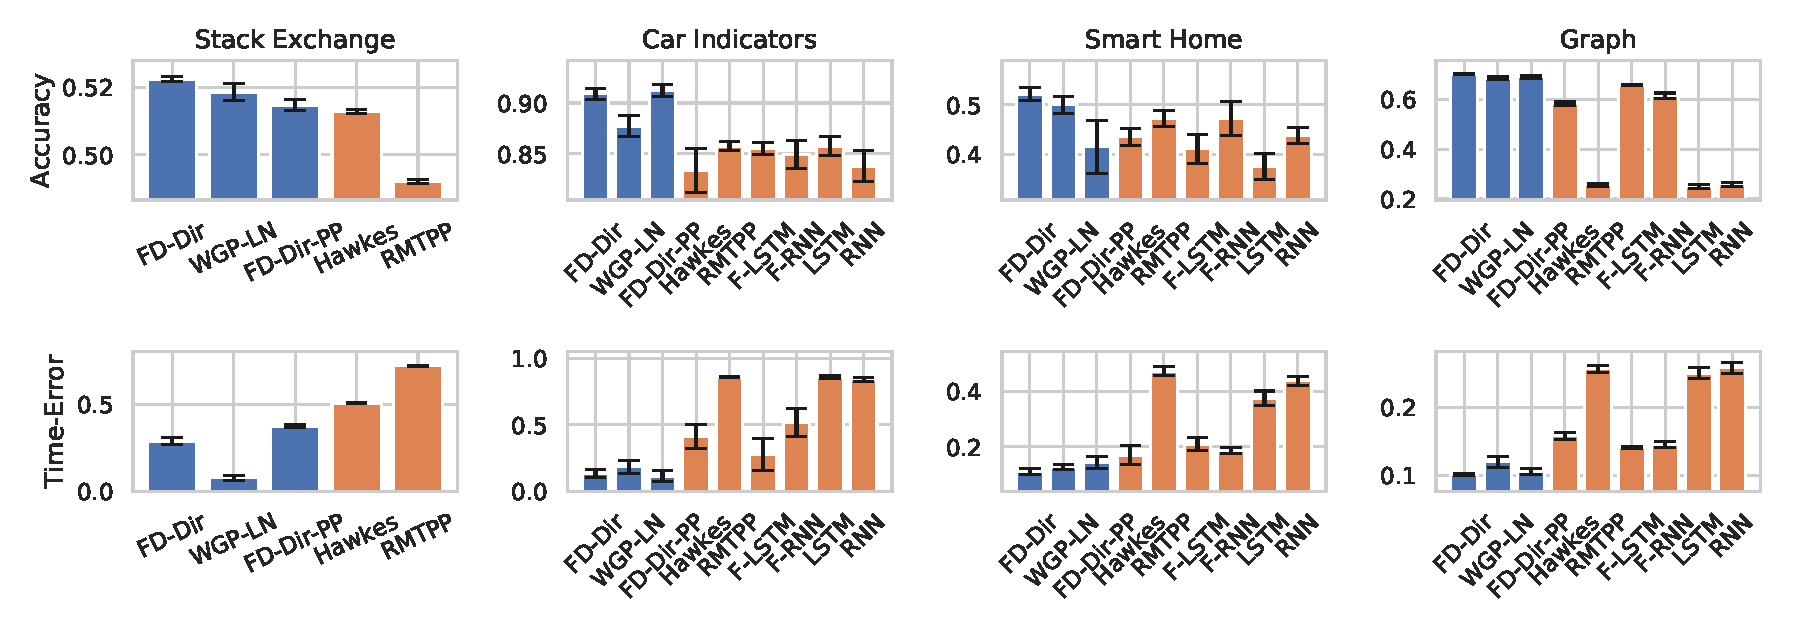
\includegraphics[width=\linewidth]{sections/010_neurips2019/paper/images/accuracy-final-all.pdf}
    \caption{Class accuracy (top) and \TimeScore (bottom) comparison across datasets}
    \label{fig:all_results}
\end{figure}

\begin{table}
    \centering
    \caption{Class accuracy comparison for all models on all datasets}\label{table:accuracy}
    \begin{tabular}{lcccc}
\toprule
{} &     Car Indicators &              Graph &         Smart Home &     Stack Exchange \\
\midrule
FD-Dir &  0.909 $\pm$ 0.005 &  \textbf{0.701 $\pm$ 0.002} &  \textbf{0.522 $\pm$ 0.013} &  \textbf{0.522 $\pm$ 0.001} \\
Dir-PP &  \textbf{0.912 $\pm$ 0.006} &  0.691 $\pm$ 0.006 &  0.415 $\pm$ 0.054 &  0.515 $\pm$ 0.002 \\
WGP-LN &  0.877 $\pm$ 0.010 &  0.685 $\pm$ 0.005 &  0.500 $\pm$ 0.017 &  0.519 $\pm$ 0.003 \\
\midrule
Hawkes &  0.834 $\pm$ 0.022 &  0.585 $\pm$ 0.008 &  0.435 $\pm$ 0.017 &  0.513 $\pm$ 0.001 \\
RMTPP  &  0.858 $\pm$ 0.004 &  0.257 $\pm$ 0.005 &  0.472 $\pm$ 0.016 &  0.492 $\pm$ 0.000 \\
F-LSTM &  0.855 $\pm$ 0.006 &  0.657 $\pm$ 0.002 &  0.411 $\pm$ 0.029 &                  - \\
F-RNN  &  0.849 $\pm$ 0.013 &  0.615 $\pm$ 0.011 &  0.472 $\pm$ 0.035 &                  - \\
LSTM   &  0.858 $\pm$ 0.010 &  0.251 $\pm$ 0.008 &  0.375 $\pm$ 0.026 &                  - \\
RNN    &  0.838 $\pm$ 0.016 &  0.258 $\pm$ 0.008 &  0.437 $\pm$ 0.017 &                  - \\
\bottomrule
\end{tabular}

\end{table}
\begin{table}
    \centering
    \caption{\TimeScore comparison for all models on all datasets}\label{table:time_error}
    \begin{tabular}{lcccc}
\toprule
{} &     Car Indicators &              Graph &         Smart Home &     Stack Exchange \\
\midrule
FD-Dir    &  \textbf{0.115 $\pm$ 0.040} &  \textbf{0.101 $\pm$ 0.001} &  \textbf{0.111 $\pm$ 0.011} &  0.289 $\pm$ 0.019 \\
WGP-LN    &  0.184 $\pm$ 0.047 &  0.120 $\pm$ 0.008 &  0.127 $\pm$ 0.010 &  \textbf{0.077 $\pm$ 0.016} \\
FD-Dir-PP &  0.132 $\pm$ 0.031 &  0.106 $\pm$ 0.004 &  0.143 $\pm$ 0.022 &  0.375 $\pm$ 0.007 \\
\midrule
Hawkes    &  0.412 $\pm$ 0.091 &  0.158 $\pm$ 0.005 &  0.170 $\pm$ 0.035 &  0.507 $\pm$ 0.003 \\
RMTPP     &  0.860 $\pm$ 0.004 &  0.257 $\pm$ 0.005 &  0.474 $\pm$ 0.016 &  0.721 $\pm$ 0.001 \\
F-LSTM    &  0.277 $\pm$ 0.118 &  0.141 $\pm$ 0.002 &  0.209 $\pm$ 0.023 &                  - \\
F-RNN     &  0.516 $\pm$ 0.105 &  0.146 $\pm$ 0.004 &  0.186 $\pm$ 0.011 &                  - \\
LSTM      &  0.860 $\pm$ 0.010 &  0.251 $\pm$ 0.008 &  0.376 $\pm$ 0.026 &                  - \\
RNN       &  0.841 $\pm$ 0.016 &  0.258 $\pm$ 0.008 &  0.439 $\pm$ 0.017 &                  - \\
\bottomrule
\end{tabular}

\end{table}

\subsection{Time Prediction with Point Processes}\label{time_mse}

The benefit of the point process framework is the ability to get the point estimate for the time $\hat{\tau}$ of the next event:
\begin{equation}
    \hat{\tau} = \int_0^\infty t q(\tau) dt
\end{equation}
where
\begin{equation}
q(\tau) = \lambda_0(\tau) \exp\left( -\int_0^{\tau} \lambda_0(s) ds \right)
\end{equation}
The usual way to evaluate the quality of this prediction is using an MSE score. As we have already discussed in \cref{time_prediction}, this is not optimal for our use case. Nevertheless, we did preliminary experiments comparing our neural point process model \textbf{FD-Dir-PP} to others. We use \textbf{RMTPP} \cite{RMTPP} since it achieves the best results. On Car Indicators dataset our model has mean MSE score of 0.4783 while RMTPP achieves 0.4736. At the same time FD-Dir-PP outperforms RMTPP on other tasks (see \cref{sec:experiments_010}).


% \subsubsection{Car Indicators}
% RNN\\
% \begin{tabular}{rrrrr}
\toprule
 dim &      lr &      l2 &      mean &       std \\
\midrule
  64 &  0.0010 &  0.0000 &  0.910714 &  0.006980 \\
 256 &  0.0010 &  0.0100 &  0.909524 &  0.015972 \\
  64 &  0.0010 &  0.0001 &  0.908929 &  0.006172 \\
  64 &  0.0010 &  0.0100 &  0.904167 &  0.018987 \\
  64 &  0.0100 &  0.0001 &  0.903571 &  0.014519 \\
  32 &  0.0100 &  0.0010 &  0.901786 &  0.015749 \\
  64 &  0.0100 &  0.0000 &  0.901190 &  0.016220 \\
 256 &  0.0010 &  0.0010 &  0.901190 &  0.022996 \\
  64 &  0.0010 &  0.0010 &  0.900595 &  0.010005 \\
 128 &  0.0010 &  0.0100 &  0.898810 &  0.015176 \\
  64 &  0.0100 &  0.0100 &  0.897619 &  0.018054 \\
  32 &  0.0100 &  0.0000 &  0.896429 &  0.022899 \\
 256 &  0.0001 &  0.0100 &  0.895238 &  0.016220 \\
 256 &  0.0010 &  0.0001 &  0.893452 &  0.017532 \\
  32 &  0.0100 &  0.0001 &  0.892262 &  0.025289 \\
 128 &  0.0100 &  0.0100 &  0.891667 &  0.018177 \\
 128 &  0.0100 &  0.0000 &  0.891071 &  0.012732 \\
  32 &  0.0100 &  0.0100 &  0.890476 &  0.014791 \\
 256 &  0.0010 &  0.0000 &  0.889881 &  0.016301 \\
 128 &  0.0010 &  0.0001 &  0.888690 &  0.015692 \\
 128 &  0.0010 &  0.0000 &  0.888095 &  0.015972 \\
  32 &  0.0010 &  0.0010 &  0.886905 &  0.011136 \\
 128 &  0.0010 &  0.0010 &  0.886905 &  0.015176 \\
  32 &  0.0010 &  0.0001 &  0.885119 &  0.011641 \\
  32 &  0.0010 &  0.0000 &  0.884524 &  0.011215 \\
 128 &  0.0100 &  0.0010 &  0.883929 &  0.005952 \\
 128 &  0.0100 &  0.0001 &  0.883929 &  0.017226 \\
  32 &  0.0010 &  0.0100 &  0.883333 &  0.001331 \\
 128 &  0.0001 &  0.0100 &  0.882738 &  0.007470 \\
  64 &  0.0001 &  0.0100 &  0.880952 &  0.006980 \\
  64 &  0.0100 &  0.0010 &  0.879762 &  0.005407 \\
  32 &  0.0001 &  0.0000 &  0.879762 &  0.003393 \\
  32 &  0.0001 &  0.0010 &  0.879762 &  0.003393 \\
  32 &  0.0001 &  0.0001 &  0.879762 &  0.003393 \\
 128 &  0.0001 &  0.0001 &  0.879167 &  0.003393 \\
 128 &  0.0001 &  0.0000 &  0.879167 &  0.003393 \\
  64 &  0.0001 &  0.0010 &  0.877976 &  0.003645 \\
  32 &  0.0001 &  0.0100 &  0.877976 &  0.002976 \\
 128 &  0.0001 &  0.0010 &  0.877976 &  0.002976 \\
  64 &  0.0001 &  0.0001 &  0.877381 &  0.005324 \\
  64 &  0.0001 &  0.0000 &  0.877381 &  0.005324 \\
 256 &  0.0001 &  0.0010 &  0.875000 &  0.006980 \\
 256 &  0.0001 &  0.0001 &  0.875000 &  0.006980 \\
 256 &  0.0001 &  0.0000 &  0.875000 &  0.006980 \\
 256 &  0.0100 &  0.0100 &  0.869048 &  0.031707 \\
 256 &  0.0100 &  0.0001 &  0.851190 &  0.033008 \\
 256 &  0.0100 &  0.0010 &  0.845238 &  0.024270 \\
 256 &  0.0100 &  0.0000 &  0.840476 &  0.031539 \\
\bottomrule
\end{tabular}
\vfill
% LSTM\\
% \begin{tabular}{rrrrr}
\toprule
 dim &      lr &      l2 &      mean &       std \\
\midrule
  64 &  0.0100 &  0.0010 &  0.905357 &  0.018515 \\
 128 &  0.0100 &  0.0010 &  0.901786 &  0.016571 \\
 128 &  0.0010 &  0.0001 &  0.900000 &  0.023302 \\
 128 &  0.0010 &  0.0000 &  0.898214 &  0.030234 \\
  64 &  0.0100 &  0.0001 &  0.895833 &  0.018467 \\
 256 &  0.0010 &  0.0001 &  0.895238 &  0.028962 \\
 256 &  0.0010 &  0.0010 &  0.894048 &  0.020791 \\
  32 &  0.0100 &  0.0010 &  0.892857 &  0.017981 \\
 256 &  0.0010 &  0.0000 &  0.889286 &  0.023939 \\
  64 &  0.0100 &  0.0000 &  0.888690 &  0.019471 \\
  64 &  0.0010 &  0.0010 &  0.888095 &  0.043211 \\
  32 &  0.0100 &  0.0000 &  0.881548 &  0.007986 \\
 128 &  0.0100 &  0.0000 &  0.881548 &  0.018987 \\
  64 &  0.0010 &  0.0000 &  0.880357 &  0.052629 \\
 128 &  0.0010 &  0.0010 &  0.876786 &  0.052002 \\
 128 &  0.0100 &  0.0001 &  0.873214 &  0.028901 \\
 256 &  0.0100 &  0.0000 &  0.873214 &  0.030685 \\
  64 &  0.0010 &  0.0001 &  0.872619 &  0.047451 \\
  32 &  0.0100 &  0.0001 &  0.872619 &  0.027065 \\
  64 &  0.0010 &  0.0100 &  0.857143 &  0.034580 \\
 128 &  0.0100 &  0.0100 &  0.855357 &  0.029881 \\
 256 &  0.0100 &  0.0010 &  0.854167 &  0.040535 \\
  64 &  0.0001 &  0.0001 &  0.851786 &  0.040883 \\
  32 &  0.0010 &  0.0001 &  0.849405 &  0.039066 \\
 256 &  0.0010 &  0.0100 &  0.849405 &  0.041592 \\
 256 &  0.0100 &  0.0001 &  0.846429 &  0.036970 \\
  64 &  0.0100 &  0.0100 &  0.844643 &  0.026653 \\
  64 &  0.0001 &  0.0000 &  0.844643 &  0.036414 \\
  32 &  0.0010 &  0.0010 &  0.841667 &  0.028109 \\
  64 &  0.0001 &  0.0010 &  0.839881 &  0.033301 \\
  32 &  0.0001 &  0.0001 &  0.835714 &  0.030743 \\
 128 &  0.0010 &  0.0100 &  0.835119 &  0.018658 \\
  32 &  0.0001 &  0.0000 &  0.835119 &  0.031115 \\
  32 &  0.0010 &  0.0000 &  0.832738 &  0.020447 \\
  32 &  0.0001 &  0.0010 &  0.831548 &  0.025131 \\
  64 &  0.0001 &  0.0100 &  0.830952 &  0.018152 \\
 128 &  0.0001 &  0.0100 &  0.830357 &  0.023340 \\
  32 &  0.0001 &  0.0100 &  0.829762 &  0.020338 \\
 128 &  0.0001 &  0.0010 &  0.827976 &  0.038079 \\
 256 &  0.0100 &  0.0100 &  0.822619 &  0.001630 \\
  32 &  0.0010 &  0.0100 &  0.822619 &  0.002662 \\
 256 &  0.0001 &  0.0100 &  0.822024 &  0.003880 \\
  32 &  0.0100 &  0.0100 &  0.821429 &  0.000000 \\
 256 &  0.0001 &  0.0010 &  0.801786 &  0.087244 \\
 256 &  0.0001 &  0.0000 &  0.643452 &  0.199154 \\
 128 &  0.0001 &  0.0001 &  0.642857 &  0.280852 \\
 128 &  0.0001 &  0.0000 &  0.625595 &  0.265561 \\
 256 &  0.0001 &  0.0001 &  0.623214 &  0.165019 \\
\bottomrule
\end{tabular}
\vfill
% Future-RNN\\
% \begin{tabular}{rrrrr}
\toprule
 dim &      lr &      l2 &      mean &       std \\
\midrule
  64 &  0.0010 &  0.0100 &  0.910714 &  0.014580 \\
 256 &  0.0001 &  0.0100 &  0.904762 &  0.010310 \\
 128 &  0.0010 &  0.0100 &  0.904167 &  0.018987 \\
  64 &  0.0100 &  0.0100 &  0.900595 &  0.019471 \\
  32 &  0.0010 &  0.0001 &  0.899405 &  0.015522 \\
  32 &  0.0010 &  0.0000 &  0.898810 &  0.015176 \\
 256 &  0.0010 &  0.0001 &  0.898214 &  0.013864 \\
  32 &  0.0010 &  0.0010 &  0.896429 &  0.013864 \\
  32 &  0.0100 &  0.0000 &  0.895238 &  0.010180 \\
 256 &  0.0010 &  0.0000 &  0.894643 &  0.014366 \\
 256 &  0.0010 &  0.0010 &  0.894048 &  0.016247 \\
  64 &  0.0100 &  0.0000 &  0.894048 &  0.019357 \\
  64 &  0.0010 &  0.0000 &  0.892857 &  0.018705 \\
  64 &  0.0010 &  0.0001 &  0.892857 &  0.018705 \\
  32 &  0.0010 &  0.0100 &  0.892262 &  0.010395 \\
  64 &  0.0010 &  0.0010 &  0.892262 &  0.018987 \\
 128 &  0.0010 &  0.0010 &  0.891667 &  0.021523 \\
 128 &  0.0010 &  0.0001 &  0.891667 &  0.022919 \\
 128 &  0.0010 &  0.0000 &  0.891667 &  0.022919 \\
 128 &  0.0100 &  0.0000 &  0.891667 &  0.013736 \\
  32 &  0.0100 &  0.0010 &  0.891071 &  0.010648 \\
 256 &  0.0010 &  0.0100 &  0.891071 &  0.019697 \\
 128 &  0.0100 &  0.0100 &  0.891071 &  0.017557 \\
  32 &  0.0100 &  0.0001 &  0.890476 &  0.018515 \\
  64 &  0.0100 &  0.0010 &  0.888690 &  0.014671 \\
 128 &  0.0100 &  0.0010 &  0.887500 &  0.022112 \\
  32 &  0.0100 &  0.0100 &  0.884524 &  0.005725 \\
  32 &  0.0001 &  0.0000 &  0.884524 &  0.003880 \\
  32 &  0.0001 &  0.0010 &  0.884524 &  0.003880 \\
  32 &  0.0001 &  0.0001 &  0.884524 &  0.003880 \\
  32 &  0.0001 &  0.0100 &  0.883929 &  0.003645 \\
  64 &  0.0100 &  0.0001 &  0.881548 &  0.005324 \\
 256 &  0.0100 &  0.0100 &  0.880357 &  0.003260 \\
  64 &  0.0001 &  0.0100 &  0.879762 &  0.002662 \\
  64 &  0.0001 &  0.0010 &  0.877381 &  0.006452 \\
  64 &  0.0001 &  0.0001 &  0.877381 &  0.004414 \\
  64 &  0.0001 &  0.0000 &  0.877381 &  0.004414 \\
 128 &  0.0001 &  0.0100 &  0.876190 &  0.003393 \\
 128 &  0.0100 &  0.0001 &  0.872024 &  0.024989 \\
 128 &  0.0001 &  0.0000 &  0.871429 &  0.007986 \\
 128 &  0.0001 &  0.0001 &  0.871429 &  0.007986 \\
 128 &  0.0001 &  0.0010 &  0.870833 &  0.007761 \\
 256 &  0.0001 &  0.0010 &  0.864286 &  0.014211 \\
 256 &  0.0001 &  0.0001 &  0.864286 &  0.012732 \\
 256 &  0.0001 &  0.0000 &  0.864286 &  0.012732 \\
 256 &  0.0100 &  0.0010 &  0.844048 &  0.042226 \\
 256 &  0.0100 &  0.0001 &  0.831548 &  0.027648 \\
 256 &  0.0100 &  0.0000 &  0.740476 &  0.220182 \\
\bottomrule
\end{tabular}
\vfill
% Future-LSTM\\
% \begin{tabular}{rrrrr}
\toprule
 dim &      lr &      l2 &      mean &       std \\
\midrule
 128 &  0.0010 &  0.0000 &  0.916667 &  0.007588 \\
 128 &  0.0010 &  0.0010 &  0.915476 &  0.008312 \\
 128 &  0.0010 &  0.0001 &  0.910714 &  0.013800 \\
  32 &  0.0100 &  0.0001 &  0.898810 &  0.011333 \\
  64 &  0.0010 &  0.0010 &  0.897024 &  0.034746 \\
 128 &  0.0100 &  0.0000 &  0.894643 &  0.013409 \\
  64 &  0.0100 &  0.0010 &  0.893452 &  0.018030 \\
  32 &  0.0100 &  0.0010 &  0.893452 &  0.018634 \\
 256 &  0.0010 &  0.0010 &  0.892857 &  0.015321 \\
 256 &  0.0010 &  0.0000 &  0.892262 &  0.040937 \\
  32 &  0.0100 &  0.0000 &  0.890476 &  0.012162 \\
  32 &  0.0010 &  0.0001 &  0.889881 &  0.016437 \\
  64 &  0.0100 &  0.0001 &  0.889286 &  0.022607 \\
 128 &  0.0100 &  0.0010 &  0.886310 &  0.003260 \\
 256 &  0.0100 &  0.0010 &  0.882738 &  0.039010 \\
 256 &  0.0100 &  0.0000 &  0.882143 &  0.011830 \\
  64 &  0.0010 &  0.0001 &  0.879762 &  0.047925 \\
  64 &  0.0100 &  0.0000 &  0.879167 &  0.013409 \\
  32 &  0.0010 &  0.0000 &  0.878571 &  0.033829 \\
 256 &  0.0100 &  0.0001 &  0.877976 &  0.032670 \\
  64 &  0.0010 &  0.0100 &  0.873810 &  0.033048 \\
  32 &  0.0010 &  0.0010 &  0.869048 &  0.032124 \\
 128 &  0.0100 &  0.0001 &  0.866667 &  0.026901 \\
 256 &  0.0010 &  0.0001 &  0.865476 &  0.047498 \\
  64 &  0.0010 &  0.0000 &  0.860119 &  0.050944 \\
  32 &  0.0100 &  0.0100 &  0.857143 &  0.047666 \\
  64 &  0.0100 &  0.0100 &  0.848214 &  0.032738 \\
  32 &  0.0001 &  0.0001 &  0.848214 &  0.027520 \\
  64 &  0.0001 &  0.0001 &  0.847024 &  0.026670 \\
  32 &  0.0001 &  0.0000 &  0.845833 &  0.026065 \\
  32 &  0.0010 &  0.0100 &  0.843452 &  0.029130 \\
  64 &  0.0001 &  0.0000 &  0.842857 &  0.015664 \\
 128 &  0.0001 &  0.0100 &  0.842857 &  0.031243 \\
 128 &  0.0001 &  0.0000 &  0.842262 &  0.036390 \\
 256 &  0.0010 &  0.0100 &  0.841667 &  0.018752 \\
  64 &  0.0001 &  0.0010 &  0.841667 &  0.038195 \\
  32 &  0.0001 &  0.0010 &  0.840476 &  0.028438 \\
 128 &  0.0001 &  0.0010 &  0.837500 &  0.023207 \\
 128 &  0.0100 &  0.0100 &  0.836905 &  0.028109 \\
 128 &  0.0010 &  0.0100 &  0.836905 &  0.026403 \\
 256 &  0.0001 &  0.0001 &  0.833929 &  0.025895 \\
 256 &  0.0100 &  0.0100 &  0.832143 &  0.015692 \\
 256 &  0.0001 &  0.0100 &  0.832143 &  0.016383 \\
 256 &  0.0001 &  0.0000 &  0.830952 &  0.023188 \\
  64 &  0.0001 &  0.0100 &  0.830357 &  0.016704 \\
 128 &  0.0001 &  0.0001 &  0.824405 &  0.017354 \\
 256 &  0.0001 &  0.0010 &  0.822024 &  0.021606 \\
  32 &  0.0001 &  0.0100 &  0.820833 &  0.003260 \\
\bottomrule
\end{tabular}
\vfill
% RMTPP\\
% \begin{tabular}{rrrrr}
\toprule
 dim &      lr &      l2 &      mean &       std \\
\midrule
 256 &  0.0010 &  0.0100 &  0.904762 &  0.020404 \\
 128 &  0.0010 &  0.0001 &  0.902381 &  0.016490 \\
 128 &  0.0010 &  0.0000 &  0.899405 &  0.017532 \\
  64 &  0.0100 &  0.0000 &  0.899405 &  0.015379 \\
  32 &  0.0010 &  0.0001 &  0.897024 &  0.013574 \\
  32 &  0.0010 &  0.0000 &  0.896429 &  0.018987 \\
  32 &  0.0010 &  0.0010 &  0.895238 &  0.018987 \\
  32 &  0.0100 &  0.0000 &  0.889881 &  0.011333 \\
 128 &  0.0010 &  0.0010 &  0.888095 &  0.018539 \\
  64 &  0.0100 &  0.0100 &  0.888095 &  0.019242 \\
 128 &  0.0001 &  0.0100 &  0.886905 &  0.016836 \\
 256 &  0.0001 &  0.0000 &  0.886905 &  0.012089 \\
  32 &  0.0001 &  0.0010 &  0.885714 &  0.001630 \\
  32 &  0.0001 &  0.0001 &  0.885714 &  0.002662 \\
  64 &  0.0010 &  0.0010 &  0.885119 &  0.020469 \\
  32 &  0.0001 &  0.0000 &  0.884524 &  0.002490 \\
  64 &  0.0010 &  0.0100 &  0.884524 &  0.015664 \\
  32 &  0.0001 &  0.0100 &  0.883929 &  0.002105 \\
  32 &  0.0100 &  0.0100 &  0.883929 &  0.004706 \\
  64 &  0.0010 &  0.0000 &  0.883333 &  0.011215 \\
 256 &  0.0001 &  0.0001 &  0.882738 &  0.003993 \\
 256 &  0.0010 &  0.0001 &  0.882738 &  0.015263 \\
 256 &  0.0100 &  0.0010 &  0.882143 &  0.006172 \\
  64 &  0.0001 &  0.0000 &  0.881548 &  0.009027 \\
 256 &  0.0001 &  0.0100 &  0.881548 &  0.012162 \\
 256 &  0.0001 &  0.0010 &  0.881548 &  0.001331 \\
  64 &  0.0010 &  0.0001 &  0.880357 &  0.004890 \\
  32 &  0.0100 &  0.0001 &  0.880357 &  0.016220 \\
  64 &  0.0100 &  0.0001 &  0.880357 &  0.012870 \\
  32 &  0.0010 &  0.0100 &  0.879762 &  0.005407 \\
  64 &  0.0100 &  0.0010 &  0.879762 &  0.012016 \\
 256 &  0.0010 &  0.0000 &  0.879167 &  0.006852 \\
 128 &  0.0010 &  0.0100 &  0.879167 &  0.008829 \\
 128 &  0.0001 &  0.0000 &  0.878571 &  0.033434 \\
 256 &  0.0010 &  0.0010 &  0.877976 &  0.020295 \\
 256 &  0.0100 &  0.0100 &  0.877381 &  0.011793 \\
  32 &  0.0100 &  0.0010 &  0.876786 &  0.008829 \\
 128 &  0.0001 &  0.0010 &  0.875000 &  0.030642 \\
 128 &  0.0001 &  0.0001 &  0.870238 &  0.025912 \\
  64 &  0.0001 &  0.0100 &  0.808333 &  0.162395 \\
  64 &  0.0001 &  0.0001 &  0.805357 &  0.165769 \\
  64 &  0.0001 &  0.0010 &  0.805357 &  0.165782 \\
 128 &  0.0100 &  0.0100 &  0.747024 &  0.324916 \\
 128 &  0.0100 &  0.0010 &  0.742857 &  0.322361 \\
 256 &  0.0100 &  0.0001 &  0.730952 &  0.315593 \\
 128 &  0.0100 &  0.0000 &  0.611905 &  0.406610 \\
 128 &  0.0100 &  0.0001 &  0.598214 &  0.393949 \\
 256 &  0.0100 &  0.0000 &  0.597024 &  0.393035 \\
\bottomrule
\end{tabular}
\vfill
% Hawkes\\
% \begin{tabular}{rrrrr}
\toprule
 dim &      lr &      l2 &      mean &       std \\
\midrule
 128 &  0.0100 &  0.0000 &  0.861309 &  0.029955 \\
  64 &  0.0100 &  0.0001 &  0.859524 &  0.033101 \\
  64 &  0.0100 &  0.0000 &  0.855952 &  0.026335 \\
  32 &  0.0100 &  0.0000 &  0.853571 &  0.028578 \\
 256 &  0.0100 &  0.0000 &  0.839881 &  0.011979 \\
  64 &  0.0010 &  0.0000 &  0.835714 &  0.024668 \\
 128 &  0.0100 &  0.0001 &  0.835119 &  0.016383 \\
 256 &  0.0010 &  0.0000 &  0.832738 &  0.010813 \\
  32 &  0.0100 &  0.0010 &  0.832143 &  0.019126 \\
  32 &  0.0100 &  0.0001 &  0.830952 &  0.013376 \\
  32 &  0.0010 &  0.0000 &  0.830357 &  0.018225 \\
 128 &  0.0100 &  0.0100 &  0.829167 &  0.014211 \\
 128 &  0.0010 &  0.0001 &  0.828571 &  0.008829 \\
 128 &  0.0010 &  0.0000 &  0.828571 &  0.010854 \\
  64 &  0.0100 &  0.0100 &  0.827976 &  0.009735 \\
  64 &  0.0010 &  0.0001 &  0.827976 &  0.021400 \\
 256 &  0.0100 &  0.0001 &  0.827381 &  0.009412 \\
  32 &  0.0010 &  0.0001 &  0.826786 &  0.012521 \\
 256 &  0.0010 &  0.0001 &  0.826190 &  0.009781 \\
  32 &  0.0001 &  0.0001 &  0.824405 &  0.007588 \\
  32 &  0.0001 &  0.0000 &  0.824405 &  0.004706 \\
 256 &  0.0001 &  0.0000 &  0.824405 &  0.012089 \\
  32 &  0.0100 &  0.0100 &  0.823810 &  0.001331 \\
  64 &  0.0001 &  0.0100 &  0.823214 &  0.002662 \\
  32 &  0.0001 &  0.0010 &  0.823214 &  0.005407 \\
  32 &  0.0010 &  0.0100 &  0.822619 &  0.001630 \\
  64 &  0.0100 &  0.0010 &  0.822024 &  0.001331 \\
  64 &  0.0010 &  0.0100 &  0.822024 &  0.001331 \\
 128 &  0.0100 &  0.0010 &  0.821429 &  0.002105 \\
  32 &  0.0010 &  0.0010 &  0.821429 &  0.002976 \\
 256 &  0.0100 &  0.0100 &  0.820833 &  0.002490 \\
  64 &  0.0001 &  0.0000 &  0.820238 &  0.006521 \\
 128 &  0.0001 &  0.0000 &  0.819643 &  0.002662 \\
 256 &  0.0010 &  0.0100 &  0.819048 &  0.002490 \\
 128 &  0.0010 &  0.0100 &  0.819048 &  0.001331 \\
  64 &  0.0010 &  0.0010 &  0.818452 &  0.004209 \\
 256 &  0.0100 &  0.0010 &  0.818452 &  0.004209 \\
 256 &  0.0010 &  0.0010 &  0.818452 &  0.002104 \\
 128 &  0.0001 &  0.0001 &  0.818452 &  0.002104 \\
 128 &  0.0010 &  0.0010 &  0.817262 &  0.004514 \\
 256 &  0.0001 &  0.0010 &  0.816667 &  0.003993 \\
 256 &  0.0001 &  0.0100 &  0.814881 &  0.003260 \\
 256 &  0.0001 &  0.0001 &  0.814286 &  0.004980 \\
  64 &  0.0001 &  0.0010 &  0.811905 &  0.003260 \\
 128 &  0.0001 &  0.0100 &  0.811310 &  0.004514 \\
  64 &  0.0001 &  0.0001 &  0.794048 &  0.064742 \\
 128 &  0.0001 &  0.0010 &  0.716071 &  0.215754 \\
  32 &  0.0001 &  0.0100 &  0.694643 &  0.074214 \\
\bottomrule
\end{tabular}
\vfill
% Gaussian Process\\
% \begin{tabular}{rrrrr}
\toprule
 dim &      lr &      l2 &      mean &       std \\
\midrule
 128 &  0.0100 &  0.0000 &  0.913690 &  0.012973 \\
 128 &  0.0010 &  0.0000 &  0.910119 &  0.019448 \\
  32 &  0.0100 &  0.0000 &  0.907143 &  0.018030 \\
  32 &  0.0010 &  0.0001 &  0.905357 &  0.012870 \\
  32 &  0.0010 &  0.0000 &  0.903571 &  0.027728 \\
 128 &  0.0100 &  0.0001 &  0.901786 &  0.016836 \\
 256 &  0.0100 &  0.0000 &  0.900595 &  0.016915 \\
  32 &  0.0100 &  0.0010 &  0.899405 &  0.014791 \\
  64 &  0.0100 &  0.0010 &  0.898810 &  0.012450 \\
 128 &  0.0100 &  0.0010 &  0.898214 &  0.014791 \\
  32 &  0.0010 &  0.0010 &  0.898214 &  0.028344 \\
  32 &  0.0100 &  0.0001 &  0.898214 &  0.022607 \\
 256 &  0.0100 &  0.0001 &  0.898214 &  0.030161 \\
  32 &  0.0010 &  0.0100 &  0.895238 &  0.019562 \\
 128 &  0.0010 &  0.0100 &  0.892857 &  0.022666 \\
 256 &  0.0010 &  0.0010 &  0.892262 &  0.034606 \\
 256 &  0.0100 &  0.0010 &  0.889881 &  0.036023 \\
  64 &  0.0100 &  0.0001 &  0.889881 &  0.006980 \\
 128 &  0.0010 &  0.0010 &  0.885119 &  0.054253 \\
  64 &  0.0100 &  0.0000 &  0.884524 &  0.041794 \\
  64 &  0.0010 &  0.0010 &  0.879167 &  0.054660 \\
 128 &  0.0010 &  0.0001 &  0.876786 &  0.031609 \\
  32 &  0.0100 &  0.0100 &  0.875000 &  0.039874 \\
 256 &  0.0001 &  0.0100 &  0.873810 &  0.025654 \\
 256 &  0.0010 &  0.0000 &  0.870238 &  0.027967 \\
 256 &  0.0001 &  0.0000 &  0.867857 &  0.041805 \\
 256 &  0.0100 &  0.0100 &  0.866071 &  0.044841 \\
 256 &  0.0010 &  0.0001 &  0.865476 &  0.045205 \\
 128 &  0.0001 &  0.0010 &  0.862500 &  0.035365 \\
 256 &  0.0001 &  0.0001 &  0.861905 &  0.036548 \\
  64 &  0.0100 &  0.0100 &  0.861310 &  0.035315 \\
  64 &  0.0010 &  0.0001 &  0.860714 &  0.047869 \\
 256 &  0.0001 &  0.0010 &  0.857143 &  0.037113 \\
  64 &  0.0001 &  0.0100 &  0.855357 &  0.047786 \\
  32 &  0.0001 &  0.0010 &  0.852976 &  0.050358 \\
 256 &  0.0010 &  0.0100 &  0.852976 &  0.040404 \\
  64 &  0.0010 &  0.0000 &  0.852381 &  0.047740 \\
  32 &  0.0001 &  0.0001 &  0.851190 &  0.057016 \\
 128 &  0.0001 &  0.0001 &  0.848810 &  0.034924 \\
  32 &  0.0001 &  0.0100 &  0.848810 &  0.020555 \\
  32 &  0.0001 &  0.0000 &  0.848810 &  0.050613 \\
 128 &  0.0001 &  0.0000 &  0.845238 &  0.035900 \\
  64 &  0.0001 &  0.0001 &  0.845238 &  0.049399 \\
  64 &  0.0010 &  0.0100 &  0.845238 &  0.049130 \\
 128 &  0.0100 &  0.0100 &  0.842857 &  0.032833 \\
 128 &  0.0001 &  0.0100 &  0.841071 &  0.079571 \\
  64 &  0.0001 &  0.0000 &  0.828571 &  0.018419 \\
  64 &  0.0001 &  0.0010 &  0.826190 &  0.013409 \\
\bottomrule
\end{tabular}
\vfill
% Dirichlet\\
% \begin{tabular}{rrrrr}
\toprule
 dim &      lr &      l2 &      mean &       std \\
\midrule
 128 &  0.0010 &  0.0001 &  0.930357 &  0.001630 \\
 128 &  0.0010 &  0.0000 &  0.926786 &  0.003993 \\
  32 &  0.0010 &  0.0000 &  0.926786 &  0.004514 \\
  64 &  0.0010 &  0.0001 &  0.926786 &  0.008574 \\
  32 &  0.0100 &  0.0001 &  0.925000 &  0.012162 \\
  64 &  0.0100 &  0.0010 &  0.924405 &  0.008574 \\
 128 &  0.0100 &  0.0010 &  0.924405 &  0.011830 \\
  32 &  0.0010 &  0.0001 &  0.923810 &  0.003393 \\
  64 &  0.0010 &  0.0000 &  0.923810 &  0.012016 \\
  64 &  0.0100 &  0.0100 &  0.923214 &  0.009735 \\
  32 &  0.0100 &  0.0010 &  0.922619 &  0.008677 \\
  32 &  0.0010 &  0.0010 &  0.922024 &  0.006452 \\
  64 &  0.0100 &  0.0001 &  0.922024 &  0.007704 \\
  32 &  0.0100 &  0.0100 &  0.920833 &  0.007470 \\
  64 &  0.0100 &  0.0000 &  0.918452 &  0.015117 \\
  64 &  0.0010 &  0.0010 &  0.917857 &  0.009552 \\
  32 &  0.0010 &  0.0100 &  0.917262 &  0.002490 \\
  32 &  0.0100 &  0.0000 &  0.917262 &  0.007411 \\
 256 &  0.0010 &  0.0010 &  0.917262 &  0.003880 \\
 128 &  0.0010 &  0.0100 &  0.916071 &  0.005324 \\
  32 &  0.0001 &  0.0100 &  0.915476 &  0.004514 \\
 256 &  0.0010 &  0.0000 &  0.913690 &  0.007588 \\
  64 &  0.0010 &  0.0100 &  0.913095 &  0.013376 \\
 256 &  0.0010 &  0.0001 &  0.911310 &  0.006452 \\
 256 &  0.0010 &  0.0100 &  0.911310 &  0.002490 \\
 128 &  0.0010 &  0.0010 &  0.910714 &  0.015176 \\
  32 &  0.0001 &  0.0010 &  0.905357 &  0.033368 \\
 128 &  0.0100 &  0.0100 &  0.904167 &  0.024307 \\
  64 &  0.0001 &  0.0100 &  0.903571 &  0.004980 \\
 256 &  0.0001 &  0.0100 &  0.893452 &  0.012521 \\
  32 &  0.0001 &  0.0000 &  0.888095 &  0.044224 \\
  32 &  0.0001 &  0.0001 &  0.887500 &  0.043963 \\
 128 &  0.0001 &  0.0100 &  0.881548 &  0.050306 \\
 128 &  0.0100 &  0.0000 &  0.880952 &  0.084939 \\
  64 &  0.0001 &  0.0010 &  0.872619 &  0.058032 \\
  64 &  0.0001 &  0.0001 &  0.854167 &  0.049578 \\
 128 &  0.0100 &  0.0001 &  0.852976 &  0.086862 \\
  64 &  0.0001 &  0.0000 &  0.852381 &  0.047039 \\
 128 &  0.0001 &  0.0001 &  0.836310 &  0.024452 \\
 128 &  0.0001 &  0.0000 &  0.835714 &  0.028962 \\
 256 &  0.0001 &  0.0010 &  0.805357 &  0.070511 \\
 256 &  0.0001 &  0.0001 &  0.805357 &  0.077541 \\
 256 &  0.0001 &  0.0000 &  0.801786 &  0.078450 \\
 128 &  0.0001 &  0.0010 &  0.801190 &  0.078641 \\
 256 &  0.0100 &  0.0001 &  0.166667 &  0.000000 \\
 256 &  0.0100 &  0.0100 &  0.166667 &  0.000000 \\
 256 &  0.0100 &  0.0000 &  0.166667 &  0.000000 \\
 256 &  0.0100 &  0.0010 &  0.166667 &  0.000000 \\
\bottomrule
\end{tabular}
\vfill

% \subsubsection{Smart Home}
% RNN\\
% \begin{tabular}{rrrrr}
\toprule
 dim &      lr &      l2 &      mean &       std \\
\midrule
 256 &  0.0100 &  0.0000 &  0.377236 &  0.005300 \\
  32 &  0.0100 &  0.0100 &  0.360976 &  0.015318 \\
  32 &  0.0100 &  0.0000 &  0.359350 &  0.022560 \\
  64 &  0.0100 &  0.0100 &  0.358537 &  0.019790 \\
  32 &  0.0100 &  0.0001 &  0.357724 &  0.019706 \\
  32 &  0.0100 &  0.0010 &  0.355285 &  0.021433 \\
 256 &  0.0100 &  0.0100 &  0.354472 &  0.006029 \\
 128 &  0.0100 &  0.0100 &  0.353659 &  0.024893 \\
 128 &  0.0100 &  0.0010 &  0.337398 &  0.023174 \\
  64 &  0.0100 &  0.0010 &  0.336585 &  0.017102 \\
 256 &  0.0100 &  0.0001 &  0.331707 &  0.047197 \\
  64 &  0.0100 &  0.0001 &  0.330894 &  0.014257 \\
  64 &  0.0100 &  0.0000 &  0.330894 &  0.011353 \\
 256 &  0.0100 &  0.0010 &  0.330081 &  0.028513 \\
  32 &  0.0010 &  0.0010 &  0.328455 &  0.019997 \\
 128 &  0.0100 &  0.0000 &  0.324390 &  0.011990 \\
  32 &  0.0010 &  0.0001 &  0.324390 &  0.017102 \\
  32 &  0.0010 &  0.0100 &  0.324390 &  0.023245 \\
  32 &  0.0010 &  0.0000 &  0.324390 &  0.017579 \\
  64 &  0.0010 &  0.0100 &  0.317073 &  0.016512 \\
 128 &  0.0100 &  0.0001 &  0.312195 &  0.022154 \\
  64 &  0.0010 &  0.0001 &  0.292683 &  0.017951 \\
  64 &  0.0010 &  0.0000 &  0.291870 &  0.018043 \\
  64 &  0.0010 &  0.0010 &  0.290244 &  0.016158 \\
 128 &  0.0010 &  0.0100 &  0.280488 &  0.025548 \\
 256 &  0.0010 &  0.0100 &  0.268293 &  0.017719 \\
  32 &  0.0001 &  0.0100 &  0.260163 &  0.050364 \\
  64 &  0.0001 &  0.0100 &  0.247154 &  0.026407 \\
  32 &  0.0001 &  0.0010 &  0.240650 &  0.051048 \\
  32 &  0.0001 &  0.0000 &  0.239837 &  0.050200 \\
 256 &  0.0010 &  0.0010 &  0.239024 &  0.020608 \\
  32 &  0.0001 &  0.0001 &  0.239024 &  0.049152 \\
  64 &  0.0001 &  0.0000 &  0.233333 &  0.031303 \\
  64 &  0.0001 &  0.0001 &  0.233333 &  0.031303 \\
 128 &  0.0010 &  0.0010 &  0.233333 &  0.025965 \\
 128 &  0.0010 &  0.0001 &  0.230894 &  0.026563 \\
 128 &  0.0010 &  0.0000 &  0.229268 &  0.026438 \\
 256 &  0.0010 &  0.0000 &  0.226829 &  0.023946 \\
 256 &  0.0010 &  0.0001 &  0.225203 &  0.022742 \\
  64 &  0.0001 &  0.0010 &  0.217073 &  0.023980 \\
 128 &  0.0001 &  0.0100 &  0.210569 &  0.028945 \\
 128 &  0.0001 &  0.0001 &  0.200813 &  0.032086 \\
 128 &  0.0001 &  0.0000 &  0.200813 &  0.032086 \\
 128 &  0.0001 &  0.0010 &  0.200813 &  0.031827 \\
 256 &  0.0001 &  0.0010 &  0.194309 &  0.015046 \\
 256 &  0.0001 &  0.0000 &  0.193496 &  0.016662 \\
 256 &  0.0001 &  0.0001 &  0.193496 &  0.016662 \\
 256 &  0.0001 &  0.0100 &  0.186992 &  0.011498 \\
\bottomrule
\end{tabular}
\vfill
% LSTM\\
% \begin{tabular}{rrrrr}
\toprule
 dim &      lr &      l2 &      mean &       std \\
\midrule
  64 &  0.0100 &  0.0001 &  0.340650 &  0.026563 \\
  64 &  0.0100 &  0.0000 &  0.337398 &  0.022079 \\
  32 &  0.0100 &  0.0001 &  0.334959 &  0.030905 \\
  32 &  0.0100 &  0.0010 &  0.334146 &  0.023773 \\
  32 &  0.0100 &  0.0000 &  0.332520 &  0.029789 \\
 128 &  0.0100 &  0.0000 &  0.313008 &  0.031092 \\
 128 &  0.0100 &  0.0010 &  0.304878 &  0.017719 \\
  64 &  0.0100 &  0.0010 &  0.304878 &  0.032647 \\
 256 &  0.0100 &  0.0001 &  0.303252 &  0.015639 \\
 128 &  0.0100 &  0.0100 &  0.295122 &  0.009358 \\
 256 &  0.0100 &  0.0010 &  0.292683 &  0.029733 \\
 128 &  0.0100 &  0.0001 &  0.291057 &  0.029816 \\
  64 &  0.0100 &  0.0100 &  0.289431 &  0.017102 \\
 256 &  0.0100 &  0.0100 &  0.281301 &  0.012983 \\
  32 &  0.0100 &  0.0100 &  0.272358 &  0.014082 \\
 256 &  0.0100 &  0.0000 &  0.267480 &  0.045212 \\
 128 &  0.0010 &  0.0100 &  0.233333 &  0.006165 \\
  64 &  0.0010 &  0.0100 &  0.230081 &  0.006802 \\
  32 &  0.0010 &  0.0100 &  0.227642 &  0.017951 \\
 256 &  0.0010 &  0.0100 &  0.225203 &  0.003636 \\
  32 &  0.0010 &  0.0010 &  0.222764 &  0.024959 \\
  64 &  0.0010 &  0.0001 &  0.220325 &  0.024288 \\
 128 &  0.0010 &  0.0000 &  0.218699 &  0.045120 \\
  64 &  0.0010 &  0.0010 &  0.213821 &  0.012397 \\
  64 &  0.0010 &  0.0000 &  0.212195 &  0.019790 \\
  32 &  0.0010 &  0.0001 &  0.209756 &  0.044214 \\
 128 &  0.0010 &  0.0010 &  0.207317 &  0.012529 \\
  64 &  0.0001 &  0.0100 &  0.205691 &  0.009790 \\
 256 &  0.0010 &  0.0010 &  0.205691 &  0.014825 \\
 128 &  0.0010 &  0.0001 &  0.203252 &  0.026501 \\
  32 &  0.0001 &  0.0000 &  0.202439 &  0.006029 \\
  32 &  0.0001 &  0.0001 &  0.202439 &  0.006029 \\
 128 &  0.0001 &  0.0001 &  0.202439 &  0.004453 \\
 256 &  0.0001 &  0.0100 &  0.202439 &  0.008331 \\
  32 &  0.0001 &  0.0100 &  0.201626 &  0.004635 \\
  32 &  0.0001 &  0.0010 &  0.201626 &  0.004635 \\
 128 &  0.0001 &  0.0010 &  0.201626 &  0.003636 \\
 128 &  0.0001 &  0.0000 &  0.200813 &  0.003636 \\
 256 &  0.0001 &  0.0010 &  0.198374 &  0.003401 \\
 256 &  0.0001 &  0.0000 &  0.198374 &  0.003401 \\
 256 &  0.0001 &  0.0001 &  0.198374 &  0.003401 \\
  64 &  0.0001 &  0.0010 &  0.198374 &  0.003401 \\
 128 &  0.0001 &  0.0100 &  0.197561 &  0.013359 \\
 256 &  0.0010 &  0.0000 &  0.196748 &  0.022742 \\
 256 &  0.0010 &  0.0001 &  0.194309 &  0.016612 \\
  32 &  0.0010 &  0.0000 &  0.193496 &  0.017390 \\
  64 &  0.0001 &  0.0001 &  0.173984 &  0.049737 \\
  64 &  0.0001 &  0.0000 &  0.173984 &  0.049737 \\
\bottomrule
\end{tabular}
\vfill
% Future-RNN\\
% \begin{tabular}{rrrrr}
\toprule
 dim &      lr &      l2 &      mean &       std \\
\midrule
  32 &  0.0100 &  0.0100 &  0.395935 &  0.015901 \\
  32 &  0.0100 &  0.0010 &  0.389431 &  0.009705 \\
 256 &  0.0100 &  0.0100 &  0.385366 &  0.024959 \\
  32 &  0.0100 &  0.0000 &  0.384553 &  0.015900 \\
  32 &  0.0100 &  0.0001 &  0.383740 &  0.014825 \\
  64 &  0.0100 &  0.0100 &  0.368293 &  0.013046 \\
 256 &  0.0100 &  0.0000 &  0.365854 &  0.018179 \\
 128 &  0.0100 &  0.0100 &  0.361789 &  0.019067 \\
 256 &  0.0100 &  0.0010 &  0.359350 &  0.035157 \\
  64 &  0.0100 &  0.0000 &  0.355285 &  0.021044 \\
  64 &  0.0100 &  0.0010 &  0.353659 &  0.020926 \\
  32 &  0.0010 &  0.0100 &  0.352033 &  0.008429 \\
  64 &  0.0100 &  0.0001 &  0.351220 &  0.022376 \\
 128 &  0.0100 &  0.0001 &  0.344715 &  0.025934 \\
 256 &  0.0100 &  0.0001 &  0.342276 &  0.057517 \\
  32 &  0.0010 &  0.0010 &  0.341463 &  0.017484 \\
  32 &  0.0010 &  0.0001 &  0.337398 &  0.015479 \\
 128 &  0.0100 &  0.0000 &  0.336585 &  0.036404 \\
  32 &  0.0010 &  0.0000 &  0.335772 &  0.016412 \\
 128 &  0.0100 &  0.0010 &  0.334146 &  0.012661 \\
  64 &  0.0010 &  0.0100 &  0.323577 &  0.013964 \\
  32 &  0.0001 &  0.0010 &  0.314634 &  0.030229 \\
  32 &  0.0001 &  0.0100 &  0.311382 &  0.028542 \\
  32 &  0.0001 &  0.0001 &  0.306504 &  0.030092 \\
  32 &  0.0001 &  0.0000 &  0.306504 &  0.030092 \\
  64 &  0.0010 &  0.0010 &  0.290244 &  0.043460 \\
  64 &  0.0010 &  0.0001 &  0.288618 &  0.039307 \\
  64 &  0.0010 &  0.0000 &  0.287805 &  0.038500 \\
 256 &  0.0010 &  0.0100 &  0.284553 &  0.037367 \\
 128 &  0.0010 &  0.0100 &  0.278862 &  0.032849 \\
 128 &  0.0010 &  0.0001 &  0.257724 &  0.034083 \\
 128 &  0.0010 &  0.0000 &  0.257724 &  0.032849 \\
 128 &  0.0010 &  0.0010 &  0.256911 &  0.032444 \\
 256 &  0.0010 &  0.0000 &  0.243089 &  0.016612 \\
 256 &  0.0010 &  0.0001 &  0.241463 &  0.014825 \\
 256 &  0.0010 &  0.0010 &  0.239024 &  0.014199 \\
  64 &  0.0001 &  0.0100 &  0.230081 &  0.032723 \\
  64 &  0.0001 &  0.0010 &  0.223577 &  0.043116 \\
  64 &  0.0001 &  0.0001 &  0.222764 &  0.044101 \\
  64 &  0.0001 &  0.0000 &  0.222764 &  0.044101 \\
 128 &  0.0001 &  0.0000 &  0.208130 &  0.020807 \\
 128 &  0.0001 &  0.0010 &  0.208130 &  0.020807 \\
 128 &  0.0001 &  0.0001 &  0.208130 &  0.020807 \\
 128 &  0.0001 &  0.0100 &  0.207317 &  0.014936 \\
 256 &  0.0001 &  0.0010 &  0.204065 &  0.016612 \\
 256 &  0.0001 &  0.0001 &  0.203252 &  0.017484 \\
 256 &  0.0001 &  0.0000 &  0.203252 &  0.017484 \\
 256 &  0.0001 &  0.0100 &  0.190244 &  0.016612 \\
\bottomrule
\end{tabular}
\vfill
% Future-LSTM\\
% \begin{tabular}{rrrrr}
\toprule
 dim &      lr &      l2 &      mean &       std \\
\midrule
  32 &  0.0100 &  0.0001 &  0.352033 &  0.012059 \\
  32 &  0.0100 &  0.0000 &  0.348780 &  0.014487 \\
  64 &  0.0100 &  0.0000 &  0.343089 &  0.040303 \\
  64 &  0.0100 &  0.0001 &  0.339837 &  0.037212 \\
 256 &  0.0100 &  0.0000 &  0.325203 &  0.029030 \\
 128 &  0.0100 &  0.0010 &  0.324390 &  0.023423 \\
  32 &  0.0100 &  0.0010 &  0.322764 &  0.019196 \\
 128 &  0.0100 &  0.0000 &  0.321951 &  0.015046 \\
  64 &  0.0100 &  0.0010 &  0.317886 &  0.045937 \\
 128 &  0.0100 &  0.0001 &  0.317073 &  0.028455 \\
 256 &  0.0100 &  0.0001 &  0.317073 &  0.026187 \\
 256 &  0.0100 &  0.0010 &  0.313008 &  0.010755 \\
  64 &  0.0100 &  0.0100 &  0.300813 &  0.018849 \\
 128 &  0.0100 &  0.0100 &  0.300000 &  0.014487 \\
 256 &  0.0100 &  0.0100 &  0.293496 &  0.012983 \\
  32 &  0.0100 &  0.0100 &  0.291057 &  0.016158 \\
  32 &  0.0010 &  0.0010 &  0.238211 &  0.038842 \\
  64 &  0.0010 &  0.0100 &  0.237398 &  0.018980 \\
  64 &  0.0010 &  0.0010 &  0.235772 &  0.042635 \\
  32 &  0.0010 &  0.0100 &  0.233333 &  0.030501 \\
 256 &  0.0010 &  0.0100 &  0.230081 &  0.010600 \\
  32 &  0.0010 &  0.0001 &  0.226829 &  0.036177 \\
 128 &  0.0010 &  0.0100 &  0.226829 &  0.006029 \\
  64 &  0.0010 &  0.0000 &  0.222764 &  0.038068 \\
  64 &  0.0010 &  0.0001 &  0.222764 &  0.032698 \\
 256 &  0.0010 &  0.0010 &  0.222764 &  0.034898 \\
  32 &  0.0010 &  0.0000 &  0.220325 &  0.029650 \\
  64 &  0.0001 &  0.0100 &  0.216260 &  0.008813 \\
 256 &  0.0010 &  0.0001 &  0.216260 &  0.023423 \\
 256 &  0.0010 &  0.0000 &  0.216260 &  0.024458 \\
 256 &  0.0001 &  0.0100 &  0.212195 &  0.012330 \\
 128 &  0.0010 &  0.0001 &  0.211382 &  0.016512 \\
  32 &  0.0001 &  0.0010 &  0.209756 &  0.009358 \\
 128 &  0.0010 &  0.0000 &  0.208943 &  0.016908 \\
  32 &  0.0001 &  0.0100 &  0.204878 &  0.017858 \\
 128 &  0.0010 &  0.0010 &  0.200813 &  0.020039 \\
 256 &  0.0001 &  0.0000 &  0.198374 &  0.008813 \\
  32 &  0.0001 &  0.0001 &  0.198374 &  0.020203 \\
 256 &  0.0001 &  0.0001 &  0.198374 &  0.008813 \\
  32 &  0.0001 &  0.0000 &  0.197561 &  0.017626 \\
 256 &  0.0001 &  0.0010 &  0.197561 &  0.007385 \\
 128 &  0.0001 &  0.0100 &  0.195935 &  0.019580 \\
  64 &  0.0001 &  0.0010 &  0.195122 &  0.024559 \\
  64 &  0.0001 &  0.0000 &  0.191870 &  0.021395 \\
  64 &  0.0001 &  0.0001 &  0.191870 &  0.019368 \\
 128 &  0.0001 &  0.0010 &  0.179675 &  0.043820 \\
 128 &  0.0001 &  0.0000 &  0.176423 &  0.051064 \\
 128 &  0.0001 &  0.0001 &  0.176423 &  0.051064 \\
\bottomrule
\end{tabular}
\vfill
% RMTPP\\
% \begin{tabular}{rrrrr}
\toprule
 dim &      lr &      l2 &      mean &       std \\
\midrule
  32 &  0.0100 &  0.0000 &  0.393496 &  0.013905 \\
  64 &  0.0100 &  0.0001 &  0.391870 &  0.008429 \\
  64 &  0.0100 &  0.0000 &  0.386179 &  0.006427 \\
  32 &  0.0100 &  0.0010 &  0.384553 &  0.011711 \\
  32 &  0.0100 &  0.0001 &  0.381301 &  0.016107 \\
  64 &  0.0100 &  0.0100 &  0.380488 &  0.026903 \\
 256 &  0.0010 &  0.0000 &  0.380488 &  0.006165 \\
  64 &  0.0100 &  0.0010 &  0.378049 &  0.017484 \\
  32 &  0.0010 &  0.0000 &  0.375610 &  0.021625 \\
  64 &  0.0010 &  0.0000 &  0.373984 &  0.022815 \\
  64 &  0.0010 &  0.0001 &  0.373984 &  0.020121 \\
 256 &  0.0010 &  0.0001 &  0.373171 &  0.023245 \\
  32 &  0.0010 &  0.0001 &  0.372358 &  0.020847 \\
  64 &  0.0010 &  0.0010 &  0.372358 &  0.014257 \\
  32 &  0.0010 &  0.0010 &  0.369106 &  0.019368 \\
  32 &  0.0010 &  0.0100 &  0.369106 &  0.012660 \\
 128 &  0.0010 &  0.0100 &  0.369106 &  0.015318 \\
 128 &  0.0010 &  0.0000 &  0.368293 &  0.024827 \\
 128 &  0.0010 &  0.0001 &  0.367480 &  0.025157 \\
  64 &  0.0010 &  0.0100 &  0.364228 &  0.011711 \\
 256 &  0.0010 &  0.0010 &  0.364228 &  0.049503 \\
 128 &  0.0010 &  0.0010 &  0.364228 &  0.023980 \\
  32 &  0.0100 &  0.0100 &  0.363415 &  0.044771 \\
 256 &  0.0010 &  0.0100 &  0.361789 &  0.010364 \\
 256 &  0.0001 &  0.0100 &  0.350407 &  0.005300 \\
 256 &  0.0001 &  0.0010 &  0.343089 &  0.018539 \\
 256 &  0.0001 &  0.0000 &  0.343089 &  0.022004 \\
 256 &  0.0001 &  0.0001 &  0.338211 &  0.015046 \\
 128 &  0.0100 &  0.0000 &  0.316260 &  0.148343 \\
 128 &  0.0100 &  0.0001 &  0.312195 &  0.145162 \\
 128 &  0.0100 &  0.0010 &  0.311382 &  0.145111 \\
 128 &  0.0001 &  0.0100 &  0.308130 &  0.087252 \\
 128 &  0.0001 &  0.0001 &  0.291057 &  0.088996 \\
 128 &  0.0001 &  0.0010 &  0.290244 &  0.088903 \\
 128 &  0.0001 &  0.0000 &  0.289431 &  0.087583 \\
  64 &  0.0001 &  0.0010 &  0.279675 &  0.116455 \\
  64 &  0.0001 &  0.0001 &  0.276423 &  0.115479 \\
  64 &  0.0001 &  0.0000 &  0.276423 &  0.115479 \\
  32 &  0.0001 &  0.0000 &  0.269919 &  0.100053 \\
  32 &  0.0001 &  0.0001 &  0.268293 &  0.099074 \\
  32 &  0.0001 &  0.0010 &  0.268293 &  0.098530 \\
  64 &  0.0001 &  0.0100 &  0.262602 &  0.112456 \\
 128 &  0.0100 &  0.0100 &  0.248780 &  0.178917 \\
  32 &  0.0001 &  0.0100 &  0.247154 &  0.094873 \\
 256 &  0.0100 &  0.0100 &  0.137398 &  0.125668 \\
 256 &  0.0100 &  0.0010 &  0.122764 &  0.156343 \\
 256 &  0.0100 &  0.0000 &  0.121951 &  0.154525 \\
 256 &  0.0100 &  0.0001 &  0.121951 &  0.154525 \\
\bottomrule
\end{tabular}
\vfill
% Hawkes\\
% \begin{tabular}{rrrrr}
\toprule
 dim &      lr &      l2 &      mean &       std \\
\midrule
  64 &  0.0100 &  0.0000 &  0.389431 &  0.011641 \\
  32 &  0.0100 &  0.0001 &  0.386992 &  0.015046 \\
  64 &  0.0100 &  0.0001 &  0.384553 &  0.018539 \\
 256 &  0.0100 &  0.0000 &  0.381301 &  0.014769 \\
 256 &  0.0100 &  0.0001 &  0.378049 &  0.017247 \\
 128 &  0.0100 &  0.0001 &  0.377236 &  0.030878 \\
 256 &  0.0100 &  0.0010 &  0.375610 &  0.022004 \\
  64 &  0.0100 &  0.0010 &  0.374797 &  0.018043 \\
  32 &  0.0100 &  0.0000 &  0.372358 &  0.020847 \\
  32 &  0.0100 &  0.0010 &  0.370732 &  0.019580 \\
 128 &  0.0100 &  0.0000 &  0.366667 &  0.016612 \\
 128 &  0.0100 &  0.0010 &  0.355285 &  0.016412 \\
  32 &  0.0010 &  0.0000 &  0.328455 &  0.033199 \\
  32 &  0.0010 &  0.0001 &  0.323577 &  0.030229 \\
 128 &  0.0100 &  0.0100 &  0.322764 &  0.011711 \\
  64 &  0.0100 &  0.0100 &  0.317886 &  0.021777 \\
  32 &  0.0010 &  0.0010 &  0.313008 &  0.019706 \\
 256 &  0.0100 &  0.0100 &  0.307317 &  0.002227 \\
  32 &  0.0100 &  0.0100 &  0.307317 &  0.013665 \\
 256 &  0.0010 &  0.0001 &  0.303252 &  0.020447 \\
  64 &  0.0010 &  0.0010 &  0.296748 &  0.021510 \\
  64 &  0.0010 &  0.0001 &  0.290244 &  0.031435 \\
 256 &  0.0010 &  0.0000 &  0.288618 &  0.012855 \\
  64 &  0.0010 &  0.0000 &  0.283740 &  0.035016 \\
 256 &  0.0010 &  0.0010 &  0.282927 &  0.045775 \\
 128 &  0.0010 &  0.0000 &  0.282114 &  0.011711 \\
 128 &  0.0010 &  0.0100 &  0.276423 &  0.023528 \\
 128 &  0.0010 &  0.0010 &  0.275610 &  0.033323 \\
 128 &  0.0010 &  0.0001 &  0.275610 &  0.019580 \\
  32 &  0.0010 &  0.0100 &  0.273171 &  0.018270 \\
  64 &  0.0010 &  0.0100 &  0.272358 &  0.017484 \\
 256 &  0.0010 &  0.0100 &  0.258537 &  0.010983 \\
 256 &  0.0001 &  0.0100 &  0.248780 &  0.014487 \\
 128 &  0.0001 &  0.0100 &  0.225203 &  0.010203 \\
 256 &  0.0001 &  0.0010 &  0.215447 &  0.020926 \\
 256 &  0.0001 &  0.0000 &  0.209756 &  0.013046 \\
 128 &  0.0001 &  0.0010 &  0.205691 &  0.003636 \\
  64 &  0.0001 &  0.0010 &  0.201626 &  0.005454 \\
  64 &  0.0001 &  0.0001 &  0.201626 &  0.010203 \\
  32 &  0.0001 &  0.0000 &  0.200000 &  0.004453 \\
  32 &  0.0001 &  0.0001 &  0.200000 &  0.004453 \\
  64 &  0.0001 &  0.0000 &  0.199187 &  0.002874 \\
 256 &  0.0001 &  0.0001 &  0.199187 &  0.013172 \\
  32 &  0.0001 &  0.0010 &  0.199187 &  0.006427 \\
  64 &  0.0001 &  0.0100 &  0.198374 &  0.007272 \\
  32 &  0.0001 &  0.0100 &  0.196748 &  0.002227 \\
 128 &  0.0001 &  0.0000 &  0.176423 &  0.057746 \\
 128 &  0.0001 &  0.0001 &  0.174797 &  0.059118 \\
\bottomrule
\end{tabular}
\vfill
% Gaussian Process\\
% \begin{tabular}{rrrrr}
\toprule
 dim &      lr &      l2 &      mean &       std \\
\midrule
  64 &  0.0010 &  0.0001 &  0.413821 &  0.014769 \\
  32 &  0.0010 &  0.0010 &  0.413008 &  0.020847 \\
  64 &  0.0010 &  0.0010 &  0.408943 &  0.016908 \\
  32 &  0.0010 &  0.0000 &  0.406504 &  0.021891 \\
 256 &  0.0010 &  0.0010 &  0.405691 &  0.019368 \\
  64 &  0.0010 &  0.0100 &  0.404878 &  0.017626 \\
  64 &  0.0010 &  0.0000 &  0.404065 &  0.013964 \\
  32 &  0.0100 &  0.0010 &  0.403252 &  0.013905 \\
 256 &  0.0010 &  0.0000 &  0.402439 &  0.009533 \\
 256 &  0.0010 &  0.0001 &  0.402439 &  0.028888 \\
  32 &  0.0100 &  0.0100 &  0.400813 &  0.016908 \\
 128 &  0.0010 &  0.0001 &  0.400813 &  0.029115 \\
 256 &  0.0001 &  0.0100 &  0.400000 &  0.013665 \\
  32 &  0.0100 &  0.0001 &  0.400000 &  0.020244 \\
  64 &  0.0100 &  0.0100 &  0.400000 &  0.015372 \\
  32 &  0.0010 &  0.0001 &  0.399187 &  0.012660 \\
 256 &  0.0010 &  0.0100 &  0.399187 &  0.016612 \\
 128 &  0.0100 &  0.0100 &  0.398374 &  0.012529 \\
  64 &  0.0001 &  0.0010 &  0.398374 &  0.012195 \\
 128 &  0.0010 &  0.0010 &  0.397561 &  0.009270 \\
 128 &  0.0010 &  0.0000 &  0.395935 &  0.014257 \\
  64 &  0.0001 &  0.0100 &  0.392683 &  0.007924 \\
  64 &  0.0001 &  0.0001 &  0.391870 &  0.018315 \\
  32 &  0.0010 &  0.0100 &  0.391870 &  0.020039 \\
  32 &  0.0100 &  0.0000 &  0.391057 &  0.013297 \\
 128 &  0.0001 &  0.0100 &  0.390244 &  0.021701 \\
  64 &  0.0001 &  0.0000 &  0.390244 &  0.023174 \\
  64 &  0.0100 &  0.0000 &  0.390244 &  0.026501 \\
 128 &  0.0010 &  0.0100 &  0.389431 &  0.018043 \\
 128 &  0.0100 &  0.0001 &  0.388618 &  0.031566 \\
  64 &  0.0100 &  0.0001 &  0.388618 &  0.021625 \\
 128 &  0.0100 &  0.0010 &  0.385366 &  0.011280 \\
  32 &  0.0001 &  0.0100 &  0.384553 &  0.013665 \\
  64 &  0.0100 &  0.0010 &  0.383740 &  0.027660 \\
 128 &  0.0100 &  0.0000 &  0.382114 &  0.022450 \\
 256 &  0.0100 &  0.0100 &  0.373171 &  0.014487 \\
 256 &  0.0100 &  0.0010 &  0.370732 &  0.033570 \\
 256 &  0.0100 &  0.0000 &  0.369919 &  0.029172 \\
 256 &  0.0100 &  0.0001 &  0.360976 &  0.030065 \\
  32 &  0.0001 &  0.0001 &  0.356098 &  0.019196 \\
  32 &  0.0001 &  0.0000 &  0.353659 &  0.023174 \\
  32 &  0.0001 &  0.0010 &  0.352846 &  0.018495 \\
 256 &  0.0001 &  0.0010 &  0.274797 &  0.114926 \\
 128 &  0.0001 &  0.0010 &  0.271545 &  0.059146 \\
 128 &  0.0001 &  0.0000 &  0.260976 &  0.080093 \\
 128 &  0.0001 &  0.0001 &  0.259350 &  0.082029 \\
 256 &  0.0001 &  0.0001 &  0.240650 &  0.070783 \\
 256 &  0.0001 &  0.0000 &  0.229268 &  0.050167 \\
\bottomrule
\end{tabular}
\vfill
% Dirichlet\\
% \begin{tabular}{rrrrr}
\toprule
 dim &      lr &      l2 &      mean &           std \\
\midrule
  32 &  0.0010 &  0.0010 &  0.427642 &  2.177740e-02 \\
  32 &  0.0100 &  0.0010 &  0.416260 &  1.020318e-02 \\
  32 &  0.0100 &  0.0001 &  0.412195 &  3.259645e-02 \\
  32 &  0.0010 &  0.0001 &  0.404878 &  2.084696e-02 \\
  64 &  0.0100 &  0.0100 &  0.404065 &  1.762560e-02 \\
  32 &  0.0100 &  0.0100 &  0.403252 &  1.504615e-02 \\
  64 &  0.0010 &  0.0010 &  0.402439 &  4.978633e-03 \\
  32 &  0.0100 &  0.0000 &  0.402439 &  3.461257e-02 \\
  32 &  0.0001 &  0.0100 &  0.397561 &  2.687235e-02 \\
  64 &  0.0100 &  0.0010 &  0.397561 &  4.199011e-02 \\
  64 &  0.0010 &  0.0100 &  0.394309 &  2.696444e-02 \\
  32 &  0.0010 &  0.0000 &  0.393496 &  2.922875e-02 \\
  64 &  0.0001 &  0.0100 &  0.390244 &  2.830973e-02 \\
  32 &  0.0001 &  0.0010 &  0.390244 &  4.406400e-02 \\
  64 &  0.0100 &  0.0000 &  0.390244 &  2.917216e-02 \\
  64 &  0.0100 &  0.0001 &  0.388618 &  2.003863e-02 \\
 128 &  0.0010 &  0.0100 &  0.385366 &  2.577377e-02 \\
  64 &  0.0010 &  0.0000 &  0.385366 &  3.127706e-02 \\
  64 &  0.0010 &  0.0001 &  0.382927 &  2.252341e-02 \\
 256 &  0.0010 &  0.0100 &  0.381301 &  1.999736e-02 \\
 128 &  0.0010 &  0.0010 &  0.380488 &  7.924220e-03 \\
 128 &  0.0001 &  0.0100 &  0.371545 &  1.482486e-02 \\
  32 &  0.0010 &  0.0100 &  0.369919 &  4.978633e-03 \\
 256 &  0.0010 &  0.0010 &  0.358537 &  3.839257e-02 \\
  32 &  0.0001 &  0.0001 &  0.355285 &  1.335909e-02 \\
 128 &  0.0010 &  0.0000 &  0.354472 &  1.661204e-02 \\
 128 &  0.0010 &  0.0001 &  0.354472 &  2.561298e-02 \\
 256 &  0.0010 &  0.0000 &  0.350407 &  5.372932e-02 \\
  32 &  0.0001 &  0.0000 &  0.347154 &  2.674907e-02 \\
 256 &  0.0010 &  0.0001 &  0.347154 &  3.050135e-02 \\
  64 &  0.0001 &  0.0010 &  0.347154 &  8.801541e-02 \\
 128 &  0.0001 &  0.0010 &  0.344715 &  3.674312e-02 \\
 256 &  0.0001 &  0.0100 &  0.336585 &  4.948676e-02 \\
 128 &  0.0100 &  0.0100 &  0.312195 &  1.490657e-01 \\
 128 &  0.0001 &  0.0001 &  0.312195 &  1.476902e-02 \\
 128 &  0.0001 &  0.0000 &  0.307317 &  6.006089e-02 \\
 256 &  0.0001 &  0.0010 &  0.305691 &  2.100490e-02 \\
  64 &  0.0001 &  0.0001 &  0.291057 &  8.030899e-02 \\
 128 &  0.0100 &  0.0010 &  0.289431 &  1.362365e-01 \\
  64 &  0.0001 &  0.0000 &  0.285366 &  8.258138e-02 \\
 256 &  0.0001 &  0.0000 &  0.281301 &  2.792775e-02 \\
 256 &  0.0001 &  0.0001 &  0.276423 &  2.931342e-02 \\
 128 &  0.0100 &  0.0001 &  0.264228 &  1.196600e-01 \\
 128 &  0.0100 &  0.0000 &  0.214634 &  1.489825e-01 \\
 256 &  0.0100 &  0.0001 &  0.052846 &  7.757919e-18 \\
 256 &  0.0100 &  0.0100 &  0.052846 &  7.757919e-18 \\
 256 &  0.0100 &  0.0000 &  0.052846 &  7.757919e-18 \\
 256 &  0.0100 &  0.0010 &  0.052846 &  7.757919e-18 \\
\bottomrule
\end{tabular}
\vfill


% \subsubsection{K-Gaussians}
% RNN\\
% \begin{tabular}{rrrrr}
\toprule
Empty DataFrame
Columns: Index(['dim', 'lr', 'l2', 'mean', 'std'], dtype='object')
Index: Int64Index([], dtype='int64') \\
\bottomrule
\end{tabular}
\vfill
% LSTM\\
% \begin{tabular}{rrrrr}
\toprule
Empty DataFrame
Columns: Index(['dim', 'lr', 'l2', 'mean', 'std'], dtype='object')
Index: Int64Index([], dtype='int64') \\
\bottomrule
\end{tabular}
\vfill
% Future-RNN\\
% \begin{tabular}{rrrrr}
\toprule
Empty DataFrame
Columns: Index(['dim', 'lr', 'l2', 'mean', 'std'], dtype='object')
Index: Int64Index([], dtype='int64') \\
\bottomrule
\end{tabular}
\vfill
% Future-LSTM\\
% \begin{tabular}{rrrrr}
\toprule
Empty DataFrame
Columns: Index(['dim', 'lr', 'l2', 'mean', 'std'], dtype='object')
Index: Int64Index([], dtype='int64') \\
\bottomrule
\end{tabular}
\vfill
% RMTPP\\
% \begin{tabular}{rrrrr}
\toprule
Empty DataFrame
Columns: Index(['dim', 'lr', 'l2', 'mean', 'std'], dtype='object')
Index: Int64Index([], dtype='int64') \\
\bottomrule
\end{tabular}
\vfill
% Hawkes\\
% \begin{tabular}{rrrrr}
\toprule
Empty DataFrame
Columns: Index(['dim', 'lr', 'l2', 'mean', 'std'], dtype='object')
Index: Int64Index([], dtype='int64') \\
\bottomrule
\end{tabular}
\vfill
% Gaussian Process\\
% \begin{tabular}{rrrrr}
\toprule
 dim &      lr &      l2 &   mean &       std \\
\midrule
  64 &  0.0100 &  0.0100 &  0.822 &  0.026363 \\
  32 &  0.0100 &  0.0001 &  0.820 &  0.007906 \\
  32 &  0.0100 &  0.0000 &  0.819 &  0.008944 \\
  32 &  0.0010 &  0.0001 &  0.818 &  0.018235 \\
  32 &  0.0010 &  0.0000 &  0.817 &  0.014405 \\
  32 &  0.0010 &  0.0010 &  0.814 &  0.020433 \\
  64 &  0.0100 &  0.0001 &  0.813 &  0.010954 \\
  32 &  0.0010 &  0.0100 &  0.808 &  0.030537 \\
  32 &  0.0100 &  0.0100 &  0.807 &  0.038503 \\
  64 &  0.0100 &  0.0010 &  0.807 &  0.007583 \\
 128 &  0.0100 &  0.0001 &  0.806 &  0.004183 \\
  64 &  0.0001 &  0.0100 &  0.806 &  0.018841 \\
  32 &  0.0100 &  0.0010 &  0.805 &  0.015811 \\
 128 &  0.0001 &  0.0100 &  0.805 &  0.034278 \\
 128 &  0.0010 &  0.0001 &  0.804 &  0.025100 \\
 128 &  0.0010 &  0.0100 &  0.804 &  0.024597 \\
 128 &  0.0010 &  0.0000 &  0.803 &  0.018235 \\
  32 &  0.0001 &  0.0010 &  0.801 &  0.021036 \\
  64 &  0.0010 &  0.0100 &  0.799 &  0.030496 \\
 256 &  0.0100 &  0.0000 &  0.798 &  0.022528 \\
  32 &  0.0001 &  0.0100 &  0.798 &  0.026125 \\
 128 &  0.0100 &  0.0100 &  0.797 &  0.029707 \\
 256 &  0.0100 &  0.0001 &  0.796 &  0.042632 \\
  64 &  0.0010 &  0.0000 &  0.795 &  0.035355 \\
  32 &  0.0001 &  0.0001 &  0.795 &  0.038406 \\
  32 &  0.0001 &  0.0000 &  0.795 &  0.038406 \\
  64 &  0.0100 &  0.0000 &  0.793 &  0.030332 \\
 128 &  0.0100 &  0.0000 &  0.791 &  0.015572 \\
 128 &  0.0100 &  0.0010 &  0.790 &  0.012748 \\
 256 &  0.0100 &  0.0010 &  0.790 &  0.028062 \\
 256 &  0.0001 &  0.0010 &  0.788 &  0.033653 \\
  64 &  0.0001 &  0.0010 &  0.786 &  0.020736 \\
 128 &  0.0001 &  0.0010 &  0.786 &  0.026077 \\
  64 &  0.0001 &  0.0000 &  0.786 &  0.025348 \\
  64 &  0.0010 &  0.0001 &  0.786 &  0.033801 \\
  64 &  0.0001 &  0.0001 &  0.785 &  0.025739 \\
 256 &  0.0100 &  0.0100 &  0.784 &  0.045744 \\
 128 &  0.0010 &  0.0010 &  0.784 &  0.016733 \\
  64 &  0.0010 &  0.0010 &  0.782 &  0.037848 \\
 256 &  0.0001 &  0.0100 &  0.782 &  0.037014 \\
 256 &  0.0010 &  0.0001 &  0.780 &  0.042279 \\
 256 &  0.0010 &  0.0100 &  0.778 &  0.025397 \\
 256 &  0.0010 &  0.0010 &  0.774 &  0.024083 \\
 256 &  0.0010 &  0.0000 &  0.770 &  0.049875 \\
 256 &  0.0001 &  0.0001 &  0.758 &  0.058481 \\
 256 &  0.0001 &  0.0000 &  0.756 &  0.062789 \\
 128 &  0.0001 &  0.0001 &  0.743 &  0.100474 \\
 128 &  0.0001 &  0.0000 &  0.741 &  0.104547 \\
\bottomrule
\end{tabular}
\vfill
% Dirichlet\\
% \begin{tabular}{rrrrr}
\toprule
Empty DataFrame
Columns: Index(['dim', 'lr', 'l2', 'mean', 'std'], dtype='object')
Index: Int64Index([], dtype='int64') \\
\bottomrule
\end{tabular}
\vfill

% \subsubsection{Random Graph}
% RNN\\
% \begin{tabular}{rrrrr}
\toprule
 dim &      lr &      l2 &    mean &       std \\
\midrule
 256 &  0.0100 &  0.0100 &  0.2689 &  0.004099 \\
 128 &  0.0100 &  0.0100 &  0.2677 &  0.012926 \\
 128 &  0.0010 &  0.0100 &  0.2666 &  0.005760 \\
 256 &  0.0010 &  0.0100 &  0.2651 &  0.003362 \\
 256 &  0.0010 &  0.0010 &  0.2651 &  0.002485 \\
  32 &  0.0010 &  0.0100 &  0.2644 &  0.002382 \\
  64 &  0.0100 &  0.0100 &  0.2644 &  0.010425 \\
 128 &  0.0001 &  0.0000 &  0.2643 &  0.003213 \\
  64 &  0.0010 &  0.0100 &  0.2638 &  0.005641 \\
 256 &  0.0001 &  0.0100 &  0.2636 &  0.003190 \\
 256 &  0.0001 &  0.0010 &  0.2633 &  0.004310 \\
  64 &  0.0001 &  0.0100 &  0.2631 &  0.001084 \\
 128 &  0.0010 &  0.0001 &  0.2626 &  0.005237 \\
 128 &  0.0001 &  0.0100 &  0.2625 &  0.002318 \\
 256 &  0.0010 &  0.0001 &  0.2625 &  0.005990 \\
  32 &  0.0001 &  0.0010 &  0.2625 &  0.005420 \\
  32 &  0.0001 &  0.0001 &  0.2624 &  0.004129 \\
 128 &  0.0010 &  0.0000 &  0.2618 &  0.004685 \\
  32 &  0.0001 &  0.0000 &  0.2617 &  0.004453 \\
 256 &  0.0010 &  0.0000 &  0.2616 &  0.004669 \\
 256 &  0.0100 &  0.0000 &  0.2615 &  0.006461 \\
  32 &  0.0001 &  0.0100 &  0.2614 &  0.001557 \\
 128 &  0.0001 &  0.0010 &  0.2614 &  0.006158 \\
  64 &  0.0001 &  0.0001 &  0.2610 &  0.008682 \\
 128 &  0.0001 &  0.0001 &  0.2606 &  0.003453 \\
 128 &  0.0010 &  0.0010 &  0.2606 &  0.005447 \\
  64 &  0.0010 &  0.0010 &  0.2603 &  0.004177 \\
  64 &  0.0001 &  0.0000 &  0.2601 &  0.007162 \\
  32 &  0.0010 &  0.0001 &  0.2600 &  0.006643 \\
  32 &  0.0010 &  0.0000 &  0.2597 &  0.006261 \\
 256 &  0.0100 &  0.0010 &  0.2595 &  0.013014 \\
  64 &  0.0001 &  0.0010 &  0.2593 &  0.007294 \\
  32 &  0.0100 &  0.0100 &  0.2588 &  0.008190 \\
 256 &  0.0001 &  0.0000 &  0.2587 &  0.005032 \\
 256 &  0.0100 &  0.0001 &  0.2585 &  0.007937 \\
  64 &  0.0100 &  0.0001 &  0.2582 &  0.009156 \\
 256 &  0.0001 &  0.0001 &  0.2580 &  0.005969 \\
  32 &  0.0100 &  0.0001 &  0.2578 &  0.005143 \\
  64 &  0.0100 &  0.0000 &  0.2575 &  0.007254 \\
 128 &  0.0100 &  0.0001 &  0.2564 &  0.009154 \\
  32 &  0.0010 &  0.0010 &  0.2564 &  0.004234 \\
  64 &  0.0010 &  0.0000 &  0.2562 &  0.004631 \\
 128 &  0.0100 &  0.0010 &  0.2560 &  0.007374 \\
  64 &  0.0100 &  0.0010 &  0.2560 &  0.003708 \\
  64 &  0.0010 &  0.0001 &  0.2560 &  0.005087 \\
  32 &  0.0100 &  0.0000 &  0.2557 &  0.005707 \\
  32 &  0.0100 &  0.0010 &  0.2557 &  0.007285 \\
 128 &  0.0100 &  0.0000 &  0.2501 &  0.007917 \\
\bottomrule
\end{tabular}
\vfill
% LSTM\\
% \begin{tabular}{rrrrr}
\toprule
 dim &      lr &      l2 &    mean &       std \\
\midrule
 256 &  0.0010 &  0.0001 &  0.2662 &  0.009648 \\
 128 &  0.0010 &  0.0001 &  0.2647 &  0.009094 \\
 128 &  0.0001 &  0.0100 &  0.2637 &  0.003290 \\
 128 &  0.0010 &  0.0100 &  0.2629 &  0.003362 \\
 128 &  0.0010 &  0.0010 &  0.2627 &  0.007094 \\
 128 &  0.0010 &  0.0000 &  0.2625 &  0.000707 \\
  32 &  0.0001 &  0.0100 &  0.2622 &  0.002971 \\
  64 &  0.0010 &  0.0100 &  0.2621 &  0.001294 \\
  32 &  0.0100 &  0.0010 &  0.2619 &  0.009476 \\
  64 &  0.0010 &  0.0000 &  0.2618 &  0.004618 \\
 128 &  0.0001 &  0.0001 &  0.2613 &  0.007621 \\
 256 &  0.0100 &  0.0010 &  0.2612 &  0.008621 \\
 256 &  0.0100 &  0.0100 &  0.2612 &  0.005369 \\
 256 &  0.0001 &  0.0100 &  0.2611 &  0.003798 \\
  64 &  0.0001 &  0.0100 &  0.2610 &  0.001768 \\
 128 &  0.0001 &  0.0010 &  0.2608 &  0.003962 \\
 256 &  0.0001 &  0.0001 &  0.2606 &  0.005771 \\
  64 &  0.0001 &  0.0010 &  0.2604 &  0.003489 \\
  64 &  0.0010 &  0.0010 &  0.2604 &  0.008019 \\
  64 &  0.0001 &  0.0001 &  0.2603 &  0.006487 \\
 128 &  0.0001 &  0.0000 &  0.2601 &  0.006887 \\
 256 &  0.0001 &  0.0000 &  0.2601 &  0.005141 \\
 256 &  0.0001 &  0.0010 &  0.2594 &  0.005273 \\
 256 &  0.0010 &  0.0000 &  0.2594 &  0.009243 \\
 256 &  0.0010 &  0.0100 &  0.2591 &  0.005030 \\
  64 &  0.0100 &  0.0001 &  0.2587 &  0.006099 \\
  32 &  0.0010 &  0.0010 &  0.2586 &  0.003362 \\
  64 &  0.0001 &  0.0000 &  0.2585 &  0.006315 \\
  32 &  0.0100 &  0.0001 &  0.2584 &  0.006417 \\
 256 &  0.0010 &  0.0010 &  0.2583 &  0.009504 \\
  64 &  0.0100 &  0.0100 &  0.2582 &  0.006211 \\
 128 &  0.0100 &  0.0100 &  0.2581 &  0.007030 \\
  64 &  0.0100 &  0.0010 &  0.2580 &  0.011429 \\
  32 &  0.0100 &  0.0000 &  0.2577 &  0.003785 \\
  32 &  0.0010 &  0.0100 &  0.2573 &  0.002515 \\
  64 &  0.0010 &  0.0001 &  0.2572 &  0.007199 \\
 128 &  0.0100 &  0.0010 &  0.2570 &  0.008307 \\
  32 &  0.0001 &  0.0010 &  0.2555 &  0.005466 \\
  32 &  0.0010 &  0.0001 &  0.2552 &  0.007371 \\
  32 &  0.0001 &  0.0000 &  0.2552 &  0.007563 \\
  32 &  0.0100 &  0.0100 &  0.2548 &  0.003012 \\
  32 &  0.0010 &  0.0000 &  0.2547 &  0.009878 \\
 128 &  0.0100 &  0.0001 &  0.2546 &  0.007092 \\
 256 &  0.0100 &  0.0000 &  0.2544 &  0.009870 \\
 128 &  0.0100 &  0.0000 &  0.2543 &  0.002775 \\
  32 &  0.0001 &  0.0001 &  0.2523 &  0.006870 \\
  64 &  0.0100 &  0.0000 &  0.2517 &  0.004645 \\
 256 &  0.0100 &  0.0001 &  0.2501 &  0.005716 \\
\bottomrule
\end{tabular}
\vfill
% Future-RNN\\
% \begin{tabular}{rrrrr}
\toprule
 dim &      lr &      l2 &    mean &       std \\
\midrule
  32 &  0.0100 &  0.0001 &  0.5934 &  0.004114 \\
  32 &  0.0100 &  0.0010 &  0.5891 &  0.008532 \\
  32 &  0.0100 &  0.0000 &  0.5868 &  0.010305 \\
  32 &  0.0010 &  0.0001 &  0.5802 &  0.011049 \\
  32 &  0.0010 &  0.0000 &  0.5801 &  0.011194 \\
  32 &  0.0010 &  0.0010 &  0.5783 &  0.010545 \\
  64 &  0.0100 &  0.0010 &  0.5102 &  0.023491 \\
  64 &  0.0100 &  0.0001 &  0.4894 &  0.009470 \\
  64 &  0.0100 &  0.0000 &  0.4870 &  0.008162 \\
  32 &  0.0100 &  0.0100 &  0.4639 &  0.005237 \\
  64 &  0.0100 &  0.0100 &  0.4579 &  0.012038 \\
  32 &  0.0001 &  0.0010 &  0.4567 &  0.002950 \\
 128 &  0.0100 &  0.0100 &  0.4562 &  0.008020 \\
  32 &  0.0010 &  0.0100 &  0.4554 &  0.003399 \\
  64 &  0.0010 &  0.0100 &  0.4551 &  0.007925 \\
  32 &  0.0001 &  0.0001 &  0.4523 &  0.006241 \\
  32 &  0.0001 &  0.0000 &  0.4522 &  0.008243 \\
 256 &  0.0100 &  0.0000 &  0.4519 &  0.066747 \\
 256 &  0.0100 &  0.0100 &  0.4492 &  0.005652 \\
 256 &  0.0100 &  0.0001 &  0.4390 &  0.064418 \\
  32 &  0.0001 &  0.0100 &  0.4358 &  0.002907 \\
 128 &  0.0100 &  0.0010 &  0.4328 &  0.011273 \\
  64 &  0.0001 &  0.0100 &  0.4285 &  0.002716 \\
 256 &  0.0010 &  0.0100 &  0.4277 &  0.010952 \\
 128 &  0.0010 &  0.0100 &  0.4272 &  0.005275 \\
  64 &  0.0010 &  0.0010 &  0.4267 &  0.008715 \\
 256 &  0.0001 &  0.0100 &  0.4248 &  0.001151 \\
 128 &  0.0001 &  0.0100 &  0.4239 &  0.005973 \\
 256 &  0.0100 &  0.0010 &  0.4238 &  0.037929 \\
  64 &  0.0010 &  0.0001 &  0.4091 &  0.007004 \\
  64 &  0.0001 &  0.0010 &  0.4090 &  0.006384 \\
  64 &  0.0010 &  0.0000 &  0.4082 &  0.006760 \\
  64 &  0.0001 &  0.0001 &  0.4038 &  0.005837 \\
  64 &  0.0001 &  0.0000 &  0.4026 &  0.004321 \\
 128 &  0.0010 &  0.0010 &  0.3984 &  0.005225 \\
 256 &  0.0010 &  0.0010 &  0.3944 &  0.009781 \\
 128 &  0.0100 &  0.0001 &  0.3935 &  0.006195 \\
 128 &  0.0100 &  0.0000 &  0.3867 &  0.005922 \\
 128 &  0.0010 &  0.0001 &  0.3859 &  0.007805 \\
 128 &  0.0010 &  0.0000 &  0.3849 &  0.006309 \\
 128 &  0.0001 &  0.0010 &  0.3796 &  0.006542 \\
 256 &  0.0010 &  0.0001 &  0.3724 &  0.005332 \\
 256 &  0.0010 &  0.0000 &  0.3715 &  0.004359 \\
 128 &  0.0001 &  0.0001 &  0.3665 &  0.009572 \\
 128 &  0.0001 &  0.0000 &  0.3656 &  0.008749 \\
 256 &  0.0001 &  0.0010 &  0.3566 &  0.007757 \\
 256 &  0.0001 &  0.0000 &  0.3363 &  0.005964 \\
 256 &  0.0001 &  0.0001 &  0.3355 &  0.005327 \\
\bottomrule
\end{tabular}
\vfill
% Future-LSTM\\
% \begin{tabular}{rrrrr}
\toprule
 dim &      lr &      l2 &    mean &       std \\
\midrule
  32 &  0.0010 &  0.0010 &  0.6277 &  0.008570 \\
  32 &  0.0100 &  0.0010 &  0.6271 &  0.010796 \\
  32 &  0.0010 &  0.0001 &  0.5990 &  0.012119 \\
  32 &  0.0100 &  0.0001 &  0.5948 &  0.009196 \\
  32 &  0.0100 &  0.0000 &  0.5878 &  0.008534 \\
  32 &  0.0010 &  0.0000 &  0.5852 &  0.014759 \\
  64 &  0.0100 &  0.0010 &  0.5820 &  0.007810 \\
  64 &  0.0010 &  0.0010 &  0.5622 &  0.011568 \\
 256 &  0.0100 &  0.0010 &  0.5604 &  0.003732 \\
 128 &  0.0100 &  0.0010 &  0.5600 &  0.009414 \\
  64 &  0.0100 &  0.0001 &  0.5286 &  0.010562 \\
  64 &  0.0100 &  0.0000 &  0.5142 &  0.006704 \\
  64 &  0.0001 &  0.0010 &  0.4906 &  0.002535 \\
  64 &  0.0010 &  0.0001 &  0.4892 &  0.020367 \\
  32 &  0.0001 &  0.0001 &  0.4854 &  0.006609 \\
  32 &  0.0001 &  0.0000 &  0.4824 &  0.006138 \\
  32 &  0.0001 &  0.0010 &  0.4768 &  0.008012 \\
  64 &  0.0010 &  0.0000 &  0.4730 &  0.015859 \\
  32 &  0.0100 &  0.0100 &  0.4701 &  0.007145 \\
  64 &  0.0100 &  0.0100 &  0.4673 &  0.004132 \\
  32 &  0.0010 &  0.0100 &  0.4667 &  0.009011 \\
  64 &  0.0001 &  0.0001 &  0.4647 &  0.014994 \\
 256 &  0.0100 &  0.0100 &  0.4612 &  0.012882 \\
 128 &  0.0100 &  0.0100 &  0.4610 &  0.017040 \\
 128 &  0.0010 &  0.0010 &  0.4586 &  0.006580 \\
  64 &  0.0010 &  0.0100 &  0.4585 &  0.007591 \\
  64 &  0.0001 &  0.0000 &  0.4554 &  0.010900 \\
 256 &  0.0010 &  0.0100 &  0.4524 &  0.005424 \\
  64 &  0.0001 &  0.0100 &  0.4491 &  0.003417 \\
 128 &  0.0010 &  0.0100 &  0.4475 &  0.009981 \\
 128 &  0.0001 &  0.0010 &  0.4438 &  0.009635 \\
 128 &  0.0100 &  0.0001 &  0.4437 &  0.008482 \\
 128 &  0.0001 &  0.0100 &  0.4435 &  0.007608 \\
  32 &  0.0001 &  0.0100 &  0.4394 &  0.002043 \\
 128 &  0.0100 &  0.0000 &  0.4341 &  0.012255 \\
 256 &  0.0010 &  0.0010 &  0.4328 &  0.003801 \\
 256 &  0.0001 &  0.0100 &  0.4304 &  0.009653 \\
 256 &  0.0100 &  0.0001 &  0.4257 &  0.014087 \\
 256 &  0.0001 &  0.0010 &  0.4188 &  0.003033 \\
 256 &  0.0100 &  0.0000 &  0.4161 &  0.011589 \\
 128 &  0.0001 &  0.0001 &  0.4155 &  0.005350 \\
 128 &  0.0010 &  0.0001 &  0.4142 &  0.007488 \\
 128 &  0.0010 &  0.0000 &  0.4128 &  0.005461 \\
 128 &  0.0001 &  0.0000 &  0.4087 &  0.006330 \\
 256 &  0.0010 &  0.0001 &  0.3938 &  0.010054 \\
 256 &  0.0010 &  0.0000 &  0.3932 &  0.008693 \\
 256 &  0.0001 &  0.0001 &  0.3885 &  0.004444 \\
 256 &  0.0001 &  0.0000 &  0.3827 &  0.010384 \\
\bottomrule
\end{tabular}
\vfill
% RMTPP\\
% \begin{tabular}{rrrrr}
\toprule
 dim &      lr &      l2 &    mean &       std \\
\midrule
 256 &  0.0010 &  0.0100 &  0.2661 &  0.007980 \\
 128 &  0.0010 &  0.0001 &  0.2650 &  0.004168 \\
  64 &  0.0010 &  0.0001 &  0.2642 &  0.007242 \\
 128 &  0.0010 &  0.0000 &  0.2640 &  0.003298 \\
  64 &  0.0010 &  0.0010 &  0.2637 &  0.006979 \\
  64 &  0.0001 &  0.0010 &  0.2622 &  0.005484 \\
  64 &  0.0001 &  0.0100 &  0.2619 &  0.003863 \\
  64 &  0.0001 &  0.0001 &  0.2617 &  0.005740 \\
 128 &  0.0001 &  0.0100 &  0.2612 &  0.005007 \\
  64 &  0.0001 &  0.0000 &  0.2605 &  0.005111 \\
  64 &  0.0010 &  0.0000 &  0.2603 &  0.006563 \\
  32 &  0.0001 &  0.0010 &  0.2602 &  0.007129 \\
 256 &  0.0001 &  0.0100 &  0.2598 &  0.005933 \\
 128 &  0.0001 &  0.0001 &  0.2592 &  0.004764 \\
  32 &  0.0001 &  0.0000 &  0.2591 &  0.006768 \\
 128 &  0.0010 &  0.0010 &  0.2591 &  0.006168 \\
  64 &  0.0100 &  0.0100 &  0.2589 &  0.005447 \\
  32 &  0.0001 &  0.0100 &  0.2588 &  0.005020 \\
 256 &  0.0100 &  0.0100 &  0.2586 &  0.008649 \\
 128 &  0.0001 &  0.0000 &  0.2584 &  0.005994 \\
 128 &  0.0001 &  0.0010 &  0.2583 &  0.006714 \\
  64 &  0.0010 &  0.0100 &  0.2582 &  0.005837 \\
  32 &  0.0001 &  0.0001 &  0.2581 &  0.009106 \\
 128 &  0.0010 &  0.0100 &  0.2578 &  0.004117 \\
  32 &  0.0100 &  0.0001 &  0.2576 &  0.007701 \\
 256 &  0.0001 &  0.0010 &  0.2573 &  0.003439 \\
  32 &  0.0010 &  0.0100 &  0.2565 &  0.002372 \\
  32 &  0.0100 &  0.0000 &  0.2562 &  0.004804 \\
  32 &  0.0010 &  0.0000 &  0.2561 &  0.010365 \\
 256 &  0.0001 &  0.0001 &  0.2549 &  0.004174 \\
 256 &  0.0001 &  0.0000 &  0.2547 &  0.004438 \\
 256 &  0.0010 &  0.0010 &  0.2546 &  0.006138 \\
  32 &  0.0010 &  0.0010 &  0.2546 &  0.007940 \\
  32 &  0.0100 &  0.0100 &  0.2539 &  0.008034 \\
  32 &  0.0010 &  0.0001 &  0.2530 &  0.009500 \\
  64 &  0.0100 &  0.0010 &  0.2529 &  0.006087 \\
 256 &  0.0010 &  0.0000 &  0.2523 &  0.009563 \\
 256 &  0.0010 &  0.0001 &  0.2521 &  0.006768 \\
  32 &  0.0100 &  0.0010 &  0.2519 &  0.007805 \\
  64 &  0.0100 &  0.0001 &  0.2491 &  0.011415 \\
  64 &  0.0100 &  0.0000 &  0.2462 &  0.013017 \\
 128 &  0.0100 &  0.0100 &  0.2237 &  0.072380 \\
 128 &  0.0100 &  0.0000 &  0.2202 &  0.070828 \\
 128 &  0.0100 &  0.0001 &  0.2196 &  0.070607 \\
 128 &  0.0100 &  0.0010 &  0.2134 &  0.066638 \\
 256 &  0.0100 &  0.0000 &  0.1601 &  0.090052 \\
 256 &  0.0100 &  0.0001 &  0.1563 &  0.084980 \\
 256 &  0.0100 &  0.0010 &  0.1559 &  0.084087 \\
\bottomrule
\end{tabular}
\vfill
% Hawkes\\
% \begin{tabular}{rrrrr}
\toprule
 dim &      lr &      l2 &    mean &       std \\
\midrule
  32 &  0.0100 &  0.0001 &  0.5677 &  0.006843 \\
  64 &  0.0100 &  0.0001 &  0.5568 &  0.006760 \\
  32 &  0.0100 &  0.0000 &  0.5565 &  0.006557 \\
  64 &  0.0100 &  0.0000 &  0.5450 &  0.007802 \\
  64 &  0.0010 &  0.0001 &  0.5379 &  0.021267 \\
  64 &  0.0010 &  0.0000 &  0.5346 &  0.022362 \\
 128 &  0.0010 &  0.0001 &  0.5297 &  0.020272 \\
 128 &  0.0100 &  0.0001 &  0.5245 &  0.010654 \\
 128 &  0.0010 &  0.0000 &  0.5244 &  0.014635 \\
  64 &  0.0100 &  0.0010 &  0.5206 &  0.018178 \\
  32 &  0.0010 &  0.0001 &  0.5169 &  0.048900 \\
  32 &  0.0100 &  0.0010 &  0.5169 &  0.023217 \\
 128 &  0.0100 &  0.0000 &  0.5139 &  0.005650 \\
  32 &  0.0010 &  0.0000 &  0.5094 &  0.040866 \\
 128 &  0.0100 &  0.0010 &  0.5087 &  0.012138 \\
 256 &  0.0010 &  0.0001 &  0.5072 &  0.013022 \\
 256 &  0.0100 &  0.0010 &  0.4959 &  0.014788 \\
 256 &  0.0100 &  0.0001 &  0.4932 &  0.017261 \\
 256 &  0.0010 &  0.0000 &  0.4875 &  0.004514 \\
 128 &  0.0010 &  0.0010 &  0.4872 &  0.008657 \\
 256 &  0.0100 &  0.0000 &  0.4823 &  0.013008 \\
  64 &  0.0010 &  0.0010 &  0.4811 &  0.019298 \\
 256 &  0.0010 &  0.0010 &  0.4810 &  0.012515 \\
  32 &  0.0010 &  0.0010 &  0.4690 &  0.012674 \\
 256 &  0.0001 &  0.0001 &  0.4665 &  0.009035 \\
 256 &  0.0001 &  0.0000 &  0.4591 &  0.011945 \\
 128 &  0.0001 &  0.0000 &  0.4496 &  0.006552 \\
 128 &  0.0001 &  0.0010 &  0.4455 &  0.012762 \\
 128 &  0.0001 &  0.0001 &  0.4425 &  0.015592 \\
 256 &  0.0001 &  0.0010 &  0.4418 &  0.011563 \\
  64 &  0.0001 &  0.0001 &  0.4346 &  0.018362 \\
  64 &  0.0100 &  0.0100 &  0.4316 &  0.006731 \\
  64 &  0.0001 &  0.0000 &  0.4286 &  0.021138 \\
 256 &  0.0100 &  0.0100 &  0.4281 &  0.005716 \\
 128 &  0.0010 &  0.0100 &  0.4258 &  0.007076 \\
 256 &  0.0010 &  0.0100 &  0.4230 &  0.010943 \\
 128 &  0.0100 &  0.0100 &  0.4191 &  0.012132 \\
  64 &  0.0010 &  0.0100 &  0.4184 &  0.008713 \\
  32 &  0.0100 &  0.0100 &  0.4183 &  0.012682 \\
  64 &  0.0001 &  0.0010 &  0.4144 &  0.017195 \\
  32 &  0.0010 &  0.0100 &  0.4097 &  0.005263 \\
 256 &  0.0001 &  0.0100 &  0.4085 &  0.017889 \\
 128 &  0.0001 &  0.0100 &  0.3929 &  0.013713 \\
  32 &  0.0001 &  0.0000 &  0.3900 &  0.060758 \\
  32 &  0.0001 &  0.0001 &  0.3873 &  0.061519 \\
  32 &  0.0001 &  0.0010 &  0.3808 &  0.061996 \\
  64 &  0.0001 &  0.0100 &  0.3497 &  0.020981 \\
  32 &  0.0001 &  0.0100 &  0.3109 &  0.013301 \\
\bottomrule
\end{tabular}
\vfill
% Gaussian Process\\
% \begin{tabular}{rrrrr}
\toprule
 dim &      lr &      l2 &    mean &       std \\
\midrule
  32 &  0.0100 &  0.0100 &  0.6722 &  0.007345 \\
 256 &  0.0100 &  0.0100 &  0.6703 &  0.008044 \\
 256 &  0.0100 &  0.0010 &  0.6655 &  0.009394 \\
  32 &  0.0100 &  0.0010 &  0.6618 &  0.007285 \\
 128 &  0.0100 &  0.0010 &  0.6591 &  0.008142 \\
  64 &  0.0100 &  0.0010 &  0.6589 &  0.007119 \\
  64 &  0.0100 &  0.0100 &  0.6589 &  0.008842 \\
 128 &  0.0100 &  0.0100 &  0.6588 &  0.012824 \\
  32 &  0.0100 &  0.0001 &  0.6578 &  0.009331 \\
  32 &  0.0010 &  0.0100 &  0.6557 &  0.015348 \\
  64 &  0.0001 &  0.0000 &  0.6542 &  0.014780 \\
 128 &  0.0010 &  0.0000 &  0.6541 &  0.009270 \\
  32 &  0.0100 &  0.0000 &  0.6539 &  0.009581 \\
  64 &  0.0010 &  0.0100 &  0.6528 &  0.009602 \\
 128 &  0.0010 &  0.0010 &  0.6525 &  0.008711 \\
  32 &  0.0001 &  0.0010 &  0.6506 &  0.011887 \\
  64 &  0.0010 &  0.0010 &  0.6496 &  0.007428 \\
 256 &  0.0010 &  0.0100 &  0.6494 &  0.016806 \\
  32 &  0.0001 &  0.0100 &  0.6494 &  0.017275 \\
  64 &  0.0001 &  0.0001 &  0.6492 &  0.007759 \\
  64 &  0.0001 &  0.0010 &  0.6487 &  0.010598 \\
 128 &  0.0010 &  0.0001 &  0.6486 &  0.014046 \\
 256 &  0.0010 &  0.0010 &  0.6485 &  0.005037 \\
 128 &  0.0001 &  0.0010 &  0.6484 &  0.015978 \\
 128 &  0.0001 &  0.0000 &  0.6479 &  0.011305 \\
 128 &  0.0010 &  0.0100 &  0.6473 &  0.021813 \\
  64 &  0.0010 &  0.0001 &  0.6472 &  0.011841 \\
  32 &  0.0010 &  0.0010 &  0.6470 &  0.014513 \\
 128 &  0.0001 &  0.0001 &  0.6468 &  0.010103 \\
  32 &  0.0010 &  0.0000 &  0.6463 &  0.012711 \\
  64 &  0.0001 &  0.0100 &  0.6456 &  0.007012 \\
  32 &  0.0001 &  0.0001 &  0.6451 &  0.012973 \\
  64 &  0.0010 &  0.0000 &  0.6451 &  0.009781 \\
  32 &  0.0001 &  0.0000 &  0.6443 &  0.011982 \\
 128 &  0.0001 &  0.0100 &  0.6436 &  0.011653 \\
  32 &  0.0010 &  0.0001 &  0.6430 &  0.014013 \\
 256 &  0.0001 &  0.0010 &  0.6426 &  0.007709 \\
 256 &  0.0010 &  0.0000 &  0.6407 &  0.007138 \\
 256 &  0.0010 &  0.0001 &  0.6388 &  0.009318 \\
 256 &  0.0100 &  0.0001 &  0.6368 &  0.011574 \\
  64 &  0.0100 &  0.0000 &  0.6362 &  0.007604 \\
 256 &  0.0001 &  0.0000 &  0.6348 &  0.012612 \\
 128 &  0.0100 &  0.0000 &  0.6340 &  0.012364 \\
  64 &  0.0100 &  0.0001 &  0.6324 &  0.008940 \\
 256 &  0.0001 &  0.0100 &  0.6304 &  0.019047 \\
 256 &  0.0001 &  0.0001 &  0.6300 &  0.014392 \\
 128 &  0.0100 &  0.0001 &  0.6252 &  0.009517 \\
 256 &  0.0100 &  0.0000 &  0.6235 &  0.012831 \\
\bottomrule
\end{tabular}
\vfill
% Dirichlet\\
% \begin{tabular}{rrrrr}
\toprule
 dim &      lr &      l2 &    mean &       std \\
\midrule
  32 &  0.0001 &  0.0100 &  0.6924 &  0.003170 \\
  32 &  0.0010 &  0.0100 &  0.6898 &  0.002280 \\
  64 &  0.0001 &  0.0100 &  0.6893 &  0.003947 \\
  64 &  0.0010 &  0.0100 &  0.6892 &  0.003290 \\
 128 &  0.0010 &  0.0100 &  0.6887 &  0.004087 \\
 256 &  0.0010 &  0.0100 &  0.6870 &  0.005327 \\
  32 &  0.0100 &  0.0100 &  0.6865 &  0.008239 \\
 128 &  0.0001 &  0.0100 &  0.6864 &  0.002679 \\
  32 &  0.0001 &  0.0010 &  0.6821 &  0.003150 \\
  32 &  0.0001 &  0.0001 &  0.6818 &  0.006241 \\
  64 &  0.0100 &  0.0100 &  0.6783 &  0.002992 \\
  32 &  0.0001 &  0.0000 &  0.6779 &  0.002043 \\
  64 &  0.0001 &  0.0000 &  0.6772 &  0.007670 \\
  64 &  0.0001 &  0.0001 &  0.6766 &  0.005030 \\
  32 &  0.0010 &  0.0000 &  0.6765 &  0.002424 \\
  32 &  0.0010 &  0.0001 &  0.6753 &  0.008386 \\
  32 &  0.0100 &  0.0000 &  0.6722 &  0.005392 \\
 128 &  0.0010 &  0.0000 &  0.6715 &  0.005646 \\
  64 &  0.0010 &  0.0000 &  0.6705 &  0.006083 \\
 128 &  0.0001 &  0.0001 &  0.6699 &  0.006077 \\
  64 &  0.0100 &  0.0000 &  0.6691 &  0.009010 \\
 128 &  0.0001 &  0.0000 &  0.6689 &  0.004588 \\
 128 &  0.0100 &  0.0100 &  0.6683 &  0.035172 \\
 256 &  0.0001 &  0.0100 &  0.6679 &  0.005320 \\
  32 &  0.0100 &  0.0010 &  0.6676 &  0.010133 \\
  64 &  0.0010 &  0.0001 &  0.6660 &  0.005534 \\
  32 &  0.0100 &  0.0001 &  0.6646 &  0.008591 \\
 256 &  0.0010 &  0.0000 &  0.6633 &  0.005552 \\
 256 &  0.0001 &  0.0001 &  0.6632 &  0.005322 \\
 256 &  0.0001 &  0.0000 &  0.6632 &  0.011184 \\
  32 &  0.0010 &  0.0010 &  0.6627 &  0.006554 \\
 128 &  0.0010 &  0.0001 &  0.6605 &  0.010977 \\
  64 &  0.0100 &  0.0010 &  0.6585 &  0.003984 \\
  64 &  0.0100 &  0.0001 &  0.6574 &  0.006804 \\
  64 &  0.0001 &  0.0010 &  0.6550 &  0.006114 \\
  64 &  0.0010 &  0.0010 &  0.6491 &  0.008332 \\
 256 &  0.0010 &  0.0001 &  0.6451 &  0.006841 \\
 256 &  0.0001 &  0.0010 &  0.6436 &  0.026123 \\
 128 &  0.0001 &  0.0010 &  0.6410 &  0.008170 \\
 128 &  0.0010 &  0.0010 &  0.6303 &  0.010616 \\
 256 &  0.0010 &  0.0010 &  0.6070 &  0.014765 \\
 128 &  0.0100 &  0.0001 &  0.5404 &  0.249613 \\
 128 &  0.0100 &  0.0010 &  0.5399 &  0.249044 \\
 128 &  0.0100 &  0.0000 &  0.5361 &  0.247003 \\
 256 &  0.0100 &  0.0010 &  0.2067 &  0.250887 \\
 256 &  0.0100 &  0.0001 &  0.1996 &  0.235011 \\
 256 &  0.0100 &  0.0000 &  0.0945 &  0.000000 \\
 256 &  0.0100 &  0.0100 &  0.0945 &  0.000000 \\
\bottomrule
\end{tabular}
\vfill
